% Created 2026-04-22 Wed 22:23
% Intended LaTeX compiler: lualatex
\DocumentMetadata{lang = en, pdfversion = 2.0, pdfstandard = ua-2, pdfstandard = a-4, testphase = {phase-III, title, table, math, firstaid}}
\documentclass[11pt]{article}
\usepackage{amsmath}
\usepackage{fontspec}
\usepackage{graphicx}
\usepackage{longtable}
\usepackage{wrapfig}
\usepackage{rotating}
\usepackage[normalem]{ulem}
\usepackage{capt-of}
\usepackage{hyperref}
\usepackage[margin=1in]{geometry}
\usepackage{fontspec}
\usepackage{verbatim, multicol, tabularx,}
\usepackage{amsmath, amsthm, amssymb, stmaryrd, latexsym, bm, listings, qtree}
\usepackage{framed}
\usepackage{xcolor,colortbl}
\usepackage{media9}
\usepackage[export]{adjustbox}
\usepackage{algorithm}
\usepackage[noend]{algpseudocode}
\usepackage{tikz,pgfplots}
\usetikzlibrary{shapes.geometric}
\let\oldquote=\quote
\let\endoldquote=\endquote
\colorlet{shadecolor}{cyan!15}
\renewenvironment{quote}{\begin{shaded*}\begin{oldquote}}{\end{oldquote}\end{shaded*}}
% From https://tex.stackexchange.com/questions/7032/good-way-to-make-textcircled-numbers
\newcommand*\circled[1]{\tikz[baseline=(char.base)]{\node[shape=circle,draw,inner sep=2pt] (char) {#1};}}
\DeclareMathOperator*{\argmin}{arg\!min}
\DeclareMathOperator*{\argmax}{arg\!max}
\lstset{frame=tb, aboveskip=1mm, belowskip=0mm, showstringspaces=false, columns=flexible, basicstyle={\scriptsize\ttfamily}, numbers=left, frame=single, breaklines=true, breakatwhitespace=true}
\hypersetup{colorlinks=true,urlcolor=blue}
\usepackage{polyglossia}
\setdefaultlanguage[variant=US]{english}
\author{Christopher Simpkins}
\date{Kennesaw State University}
\title{Artificial Intelligence\\\medskip
\large Logical Agents}
\hypersetup{
 pdfauthor={Christopher Simpkins},
 pdftitle={Artificial Intelligence},
 pdfkeywords={},
 pdfsubject={Artificial Intelligence Logical Agents},
 pdfcreator={Emacs 30.2 (Org mode 9.7.11)}, 
 pdflang={English}}
\begin{document}

\maketitle
\section{Logic and AI}
\label{sec:org6d01d76}

In AI, \textbf{knowledge-based} agents use a process of \textbf{reasoning} over an internal \textbf{representation} of knowledge to decide what actions to take.
\section{Knowledge-Based Agents}
\label{sec:org4c17fa6}


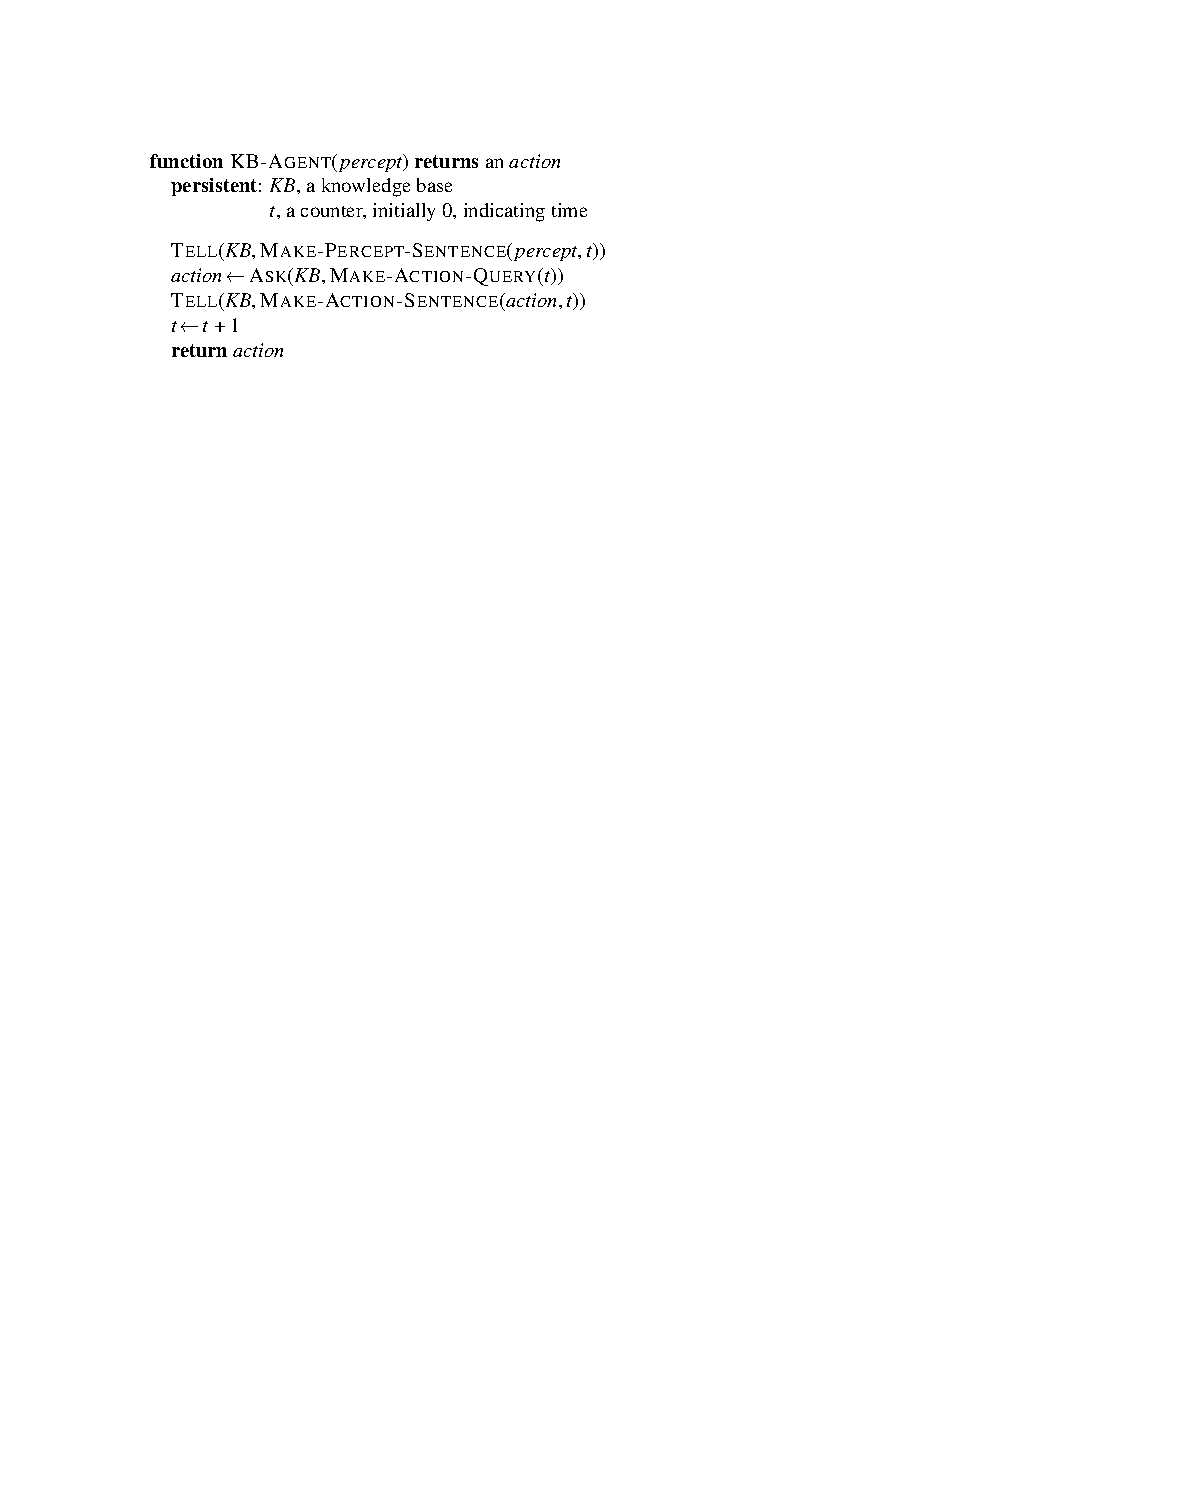
\includegraphics[alt={aima fig 07_01 kb agent},height=2.8in]{aima-fig-07_01-kb-agent.pdf}
\section{The Wumpus World}
\label{sec:orgf723e44}


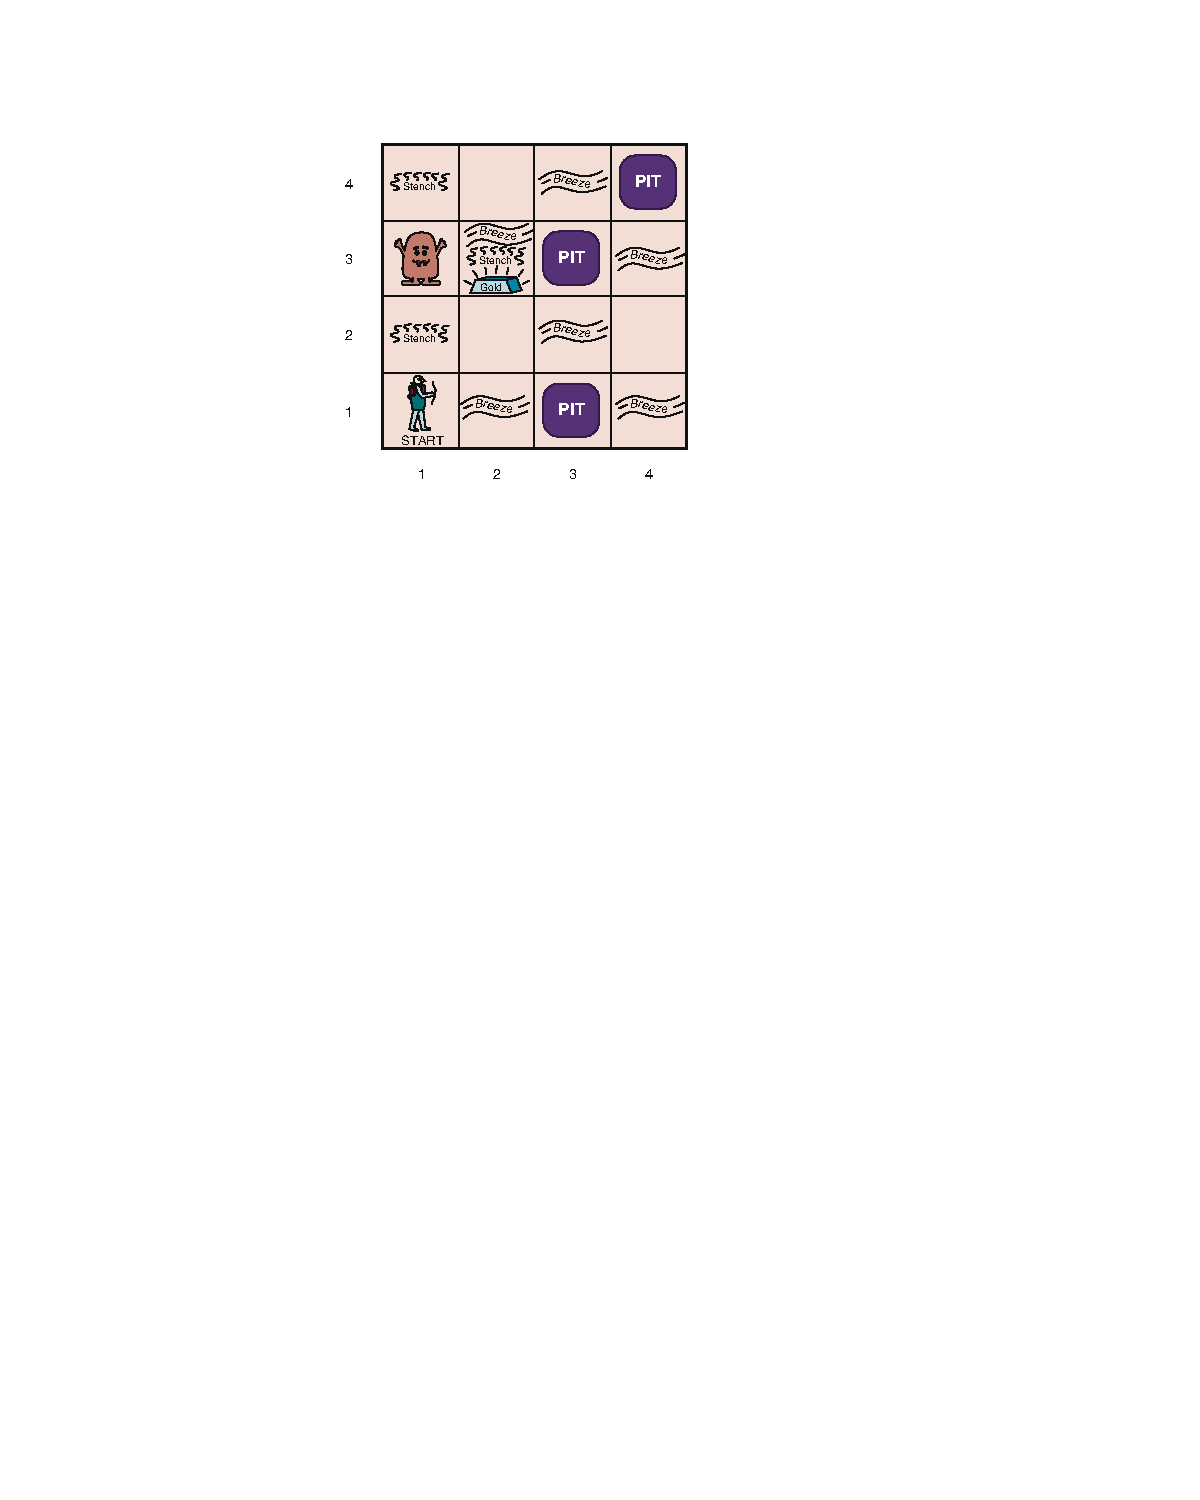
\includegraphics[alt={aima fig 07_02 wumpus world},height=2.8in]{aima-fig-07_02-wumpus-world.pdf}
\section{First Steps Wumpus WOrld}
\label{sec:orgc19fced}


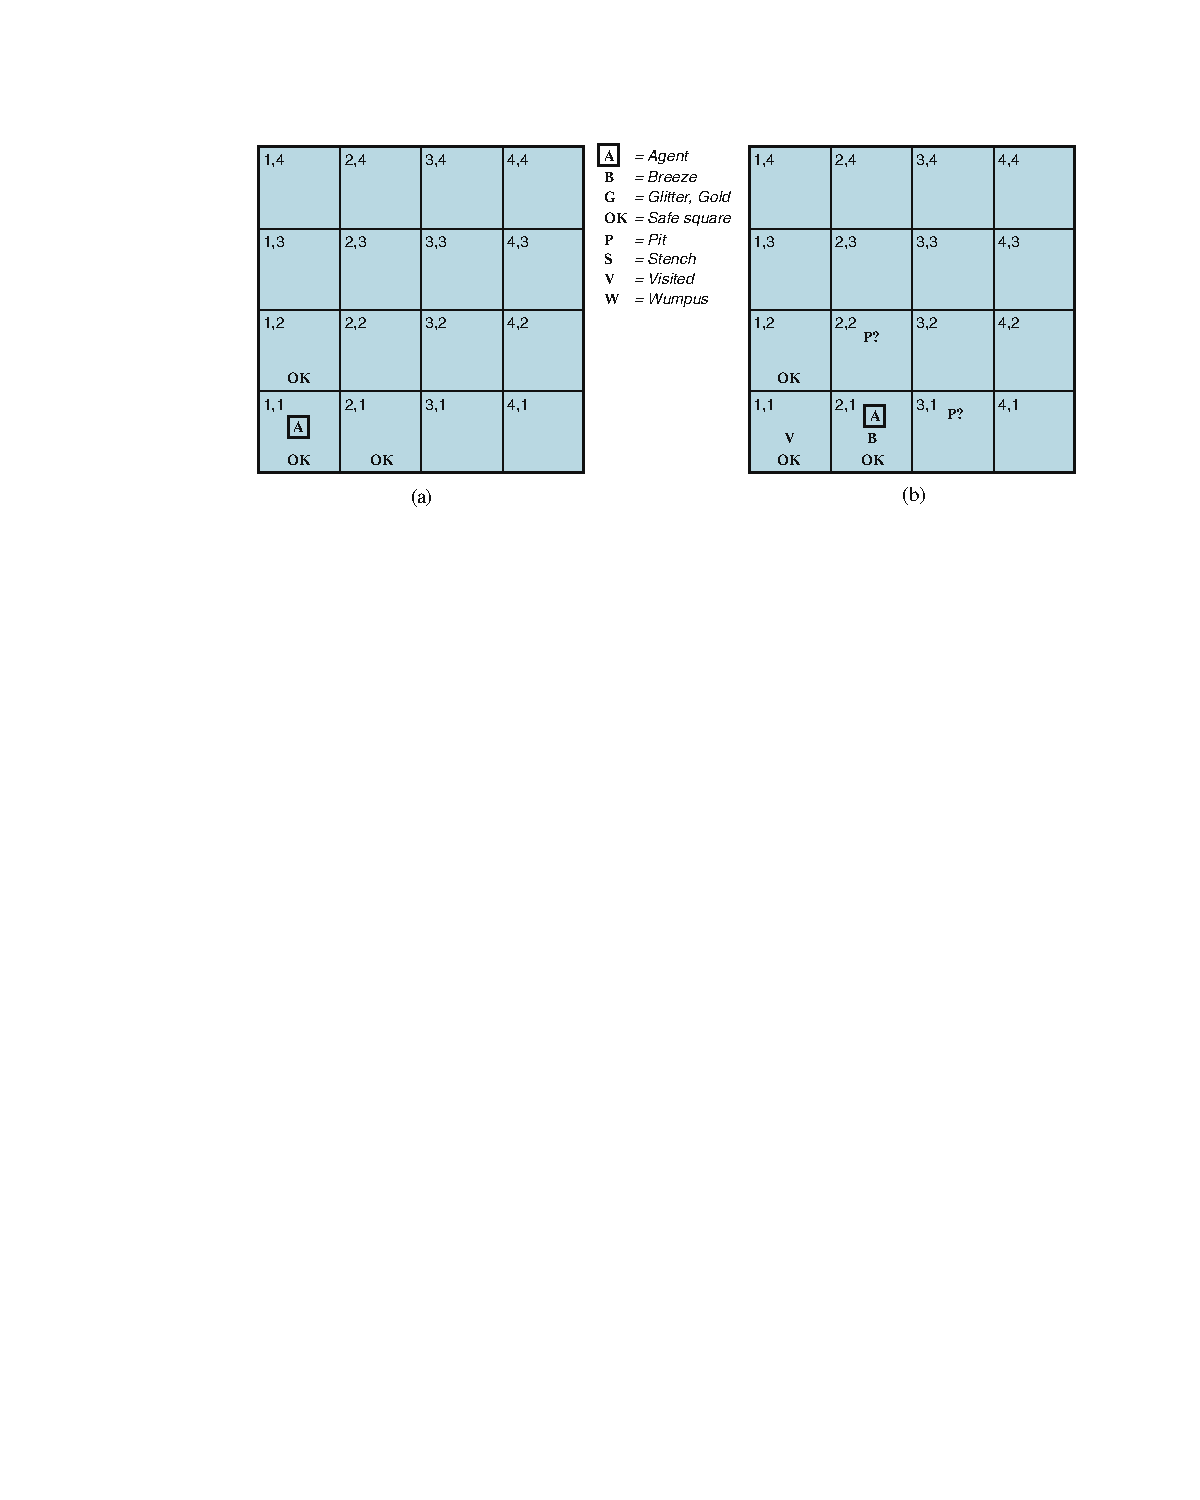
\includegraphics[alt={aima fig 07_03 first step wumpus world},height=2.8in]{aima-fig-07_03-first-step-wumpus-world.pdf}
\section{Later Steps Wumpus World}
\label{sec:orgb53c762}


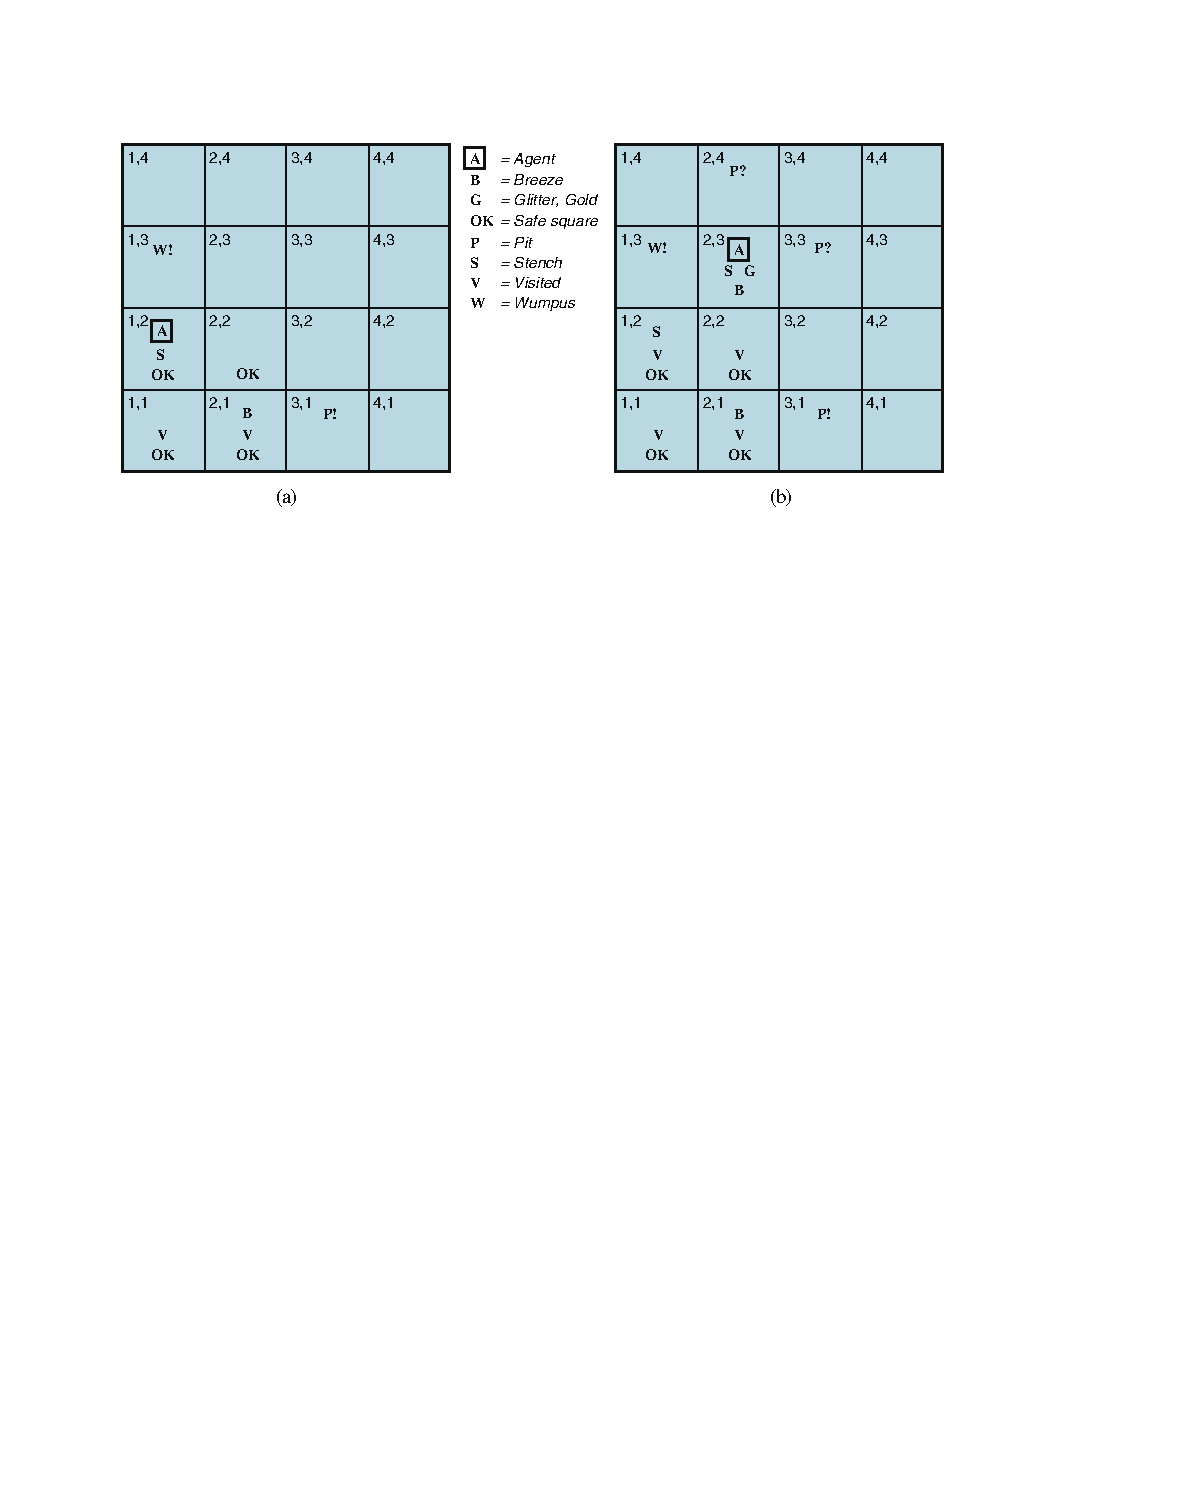
\includegraphics[alt={aima fig 07_04 later steps wumpus world},height=2.8in]{aima-fig-07_04-later-steps-wumpus-world.pdf}
\section{Logic}
\label{sec:orgb688f92}


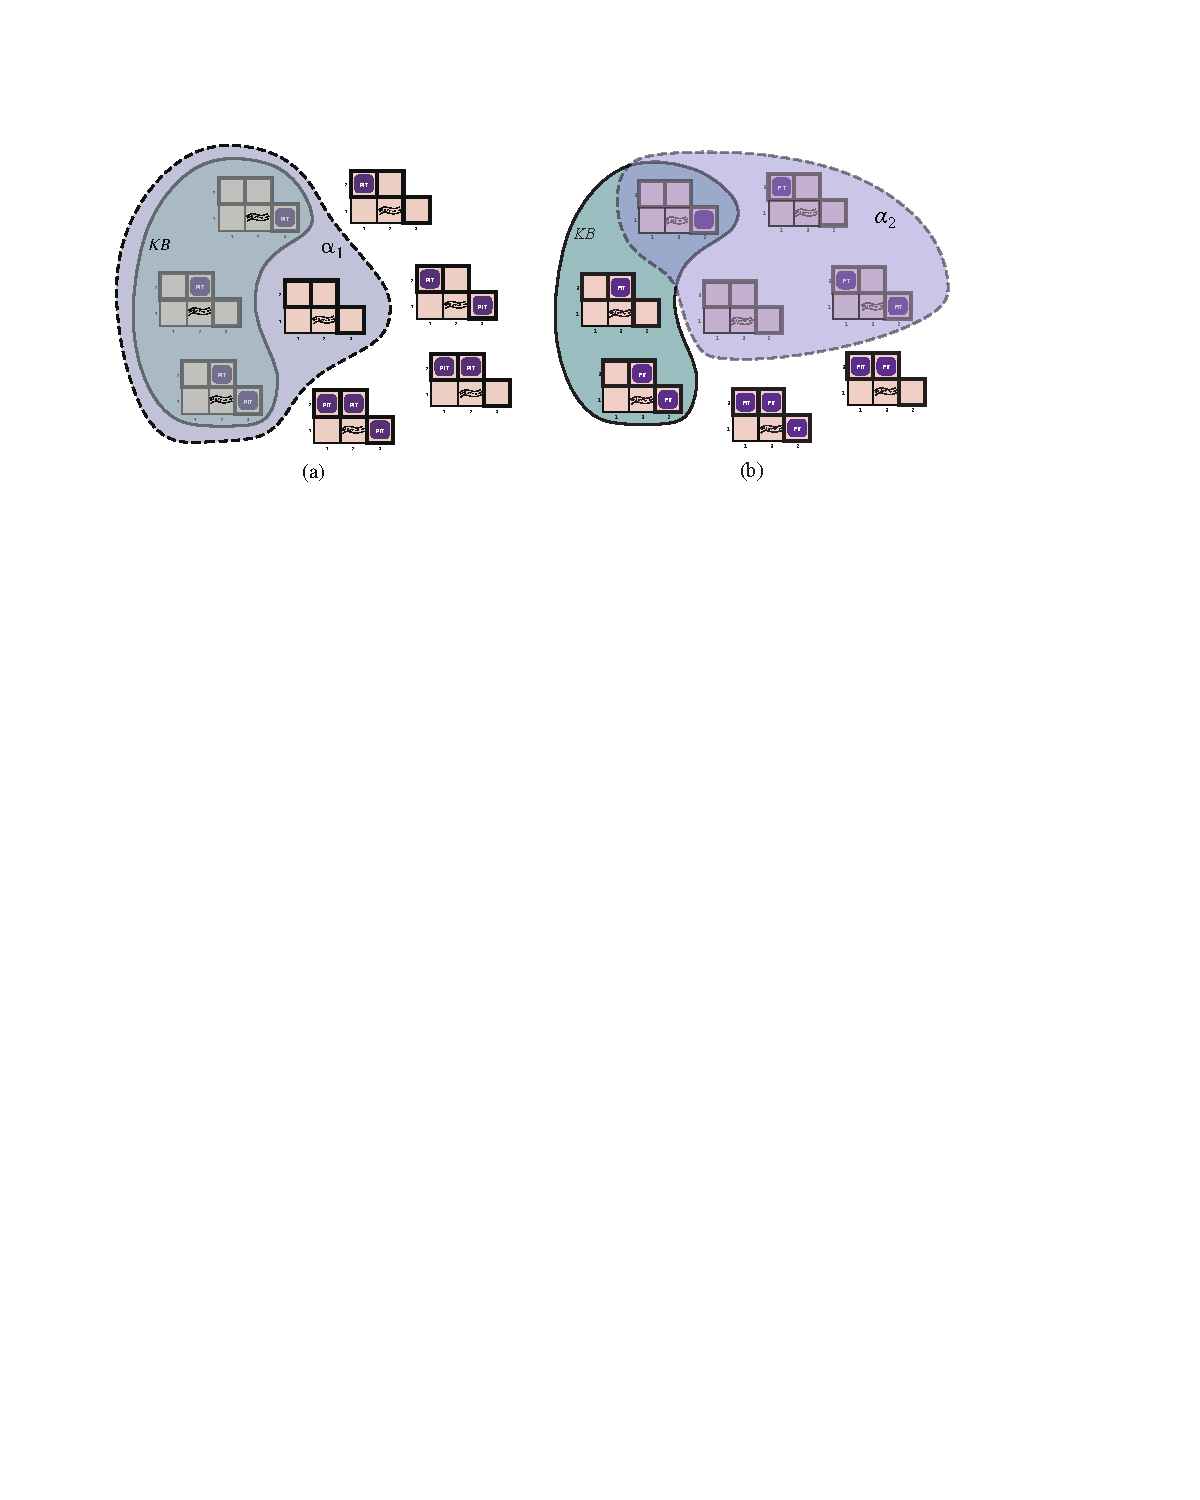
\includegraphics[alt={aima fig 07_05 possible models pits},height=2.8in]{aima-fig-07_05-possible-models-pits.pdf}
\section{Logic}
\label{sec:org2cd7ae8}


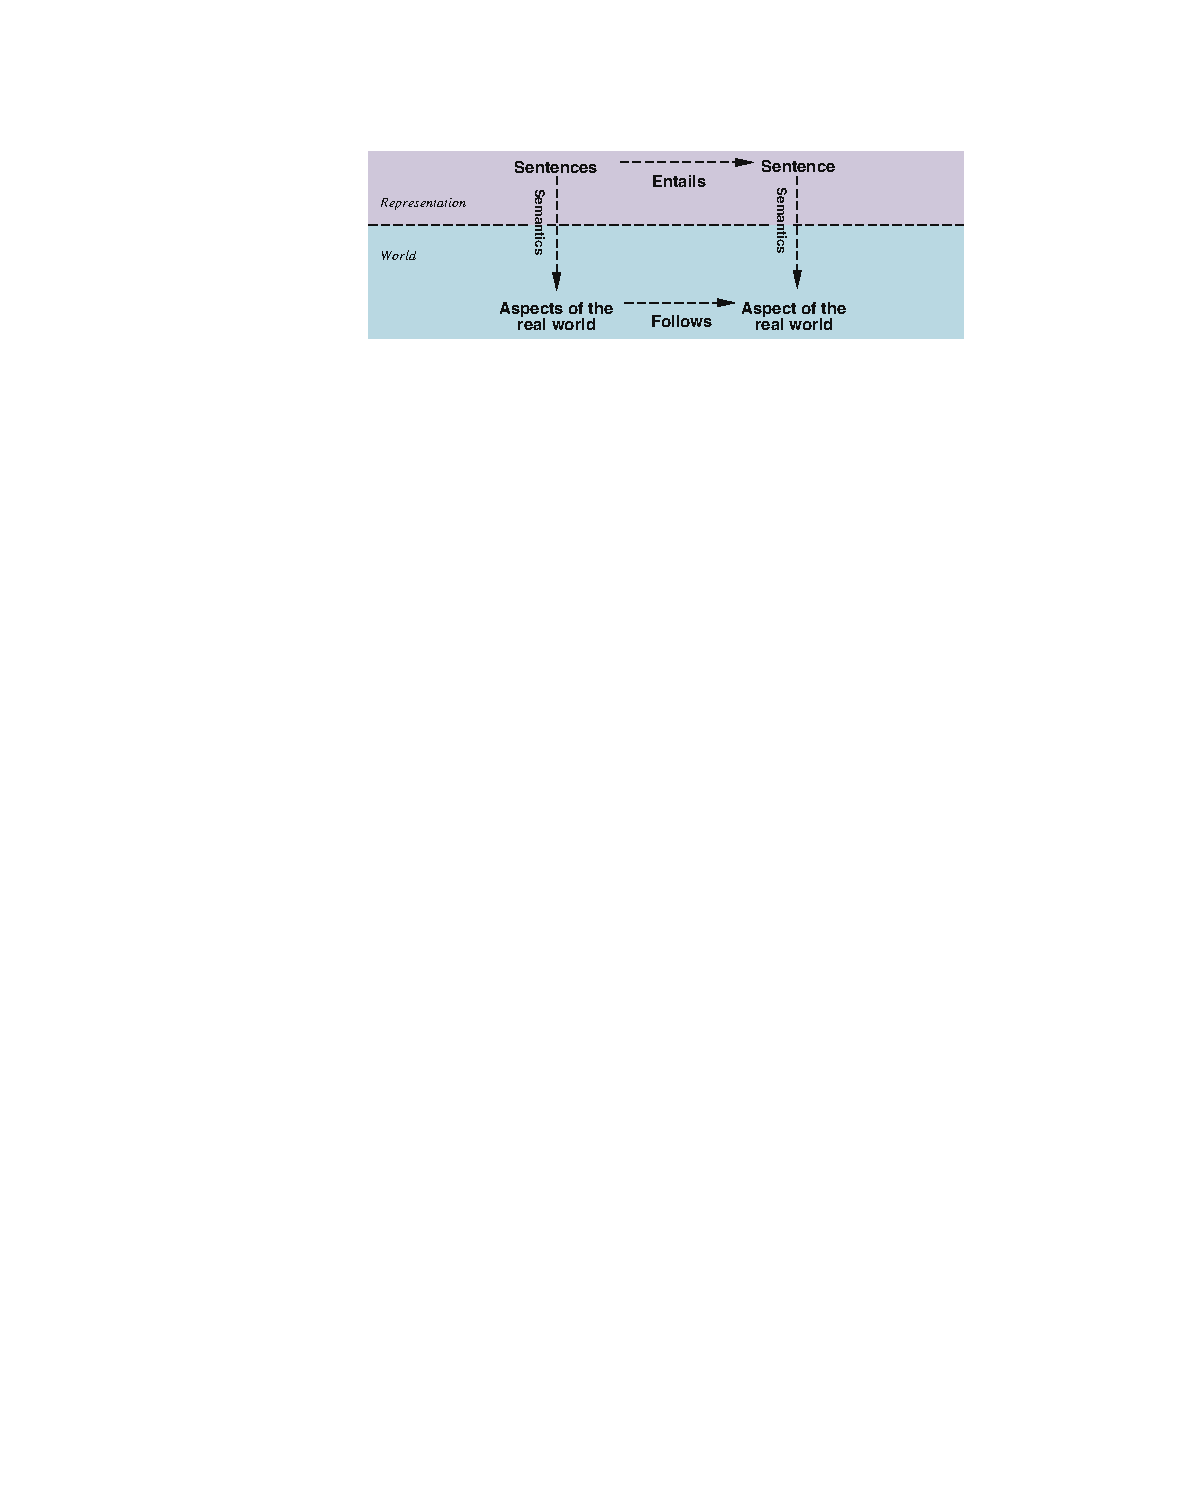
\includegraphics[alt={aima fig 07_06 representation vs world},height=2.8in]{aima-fig-07_06-representation-vs-world.pdf}
\section{Propositional Logic}
\label{sec:org92727c1}


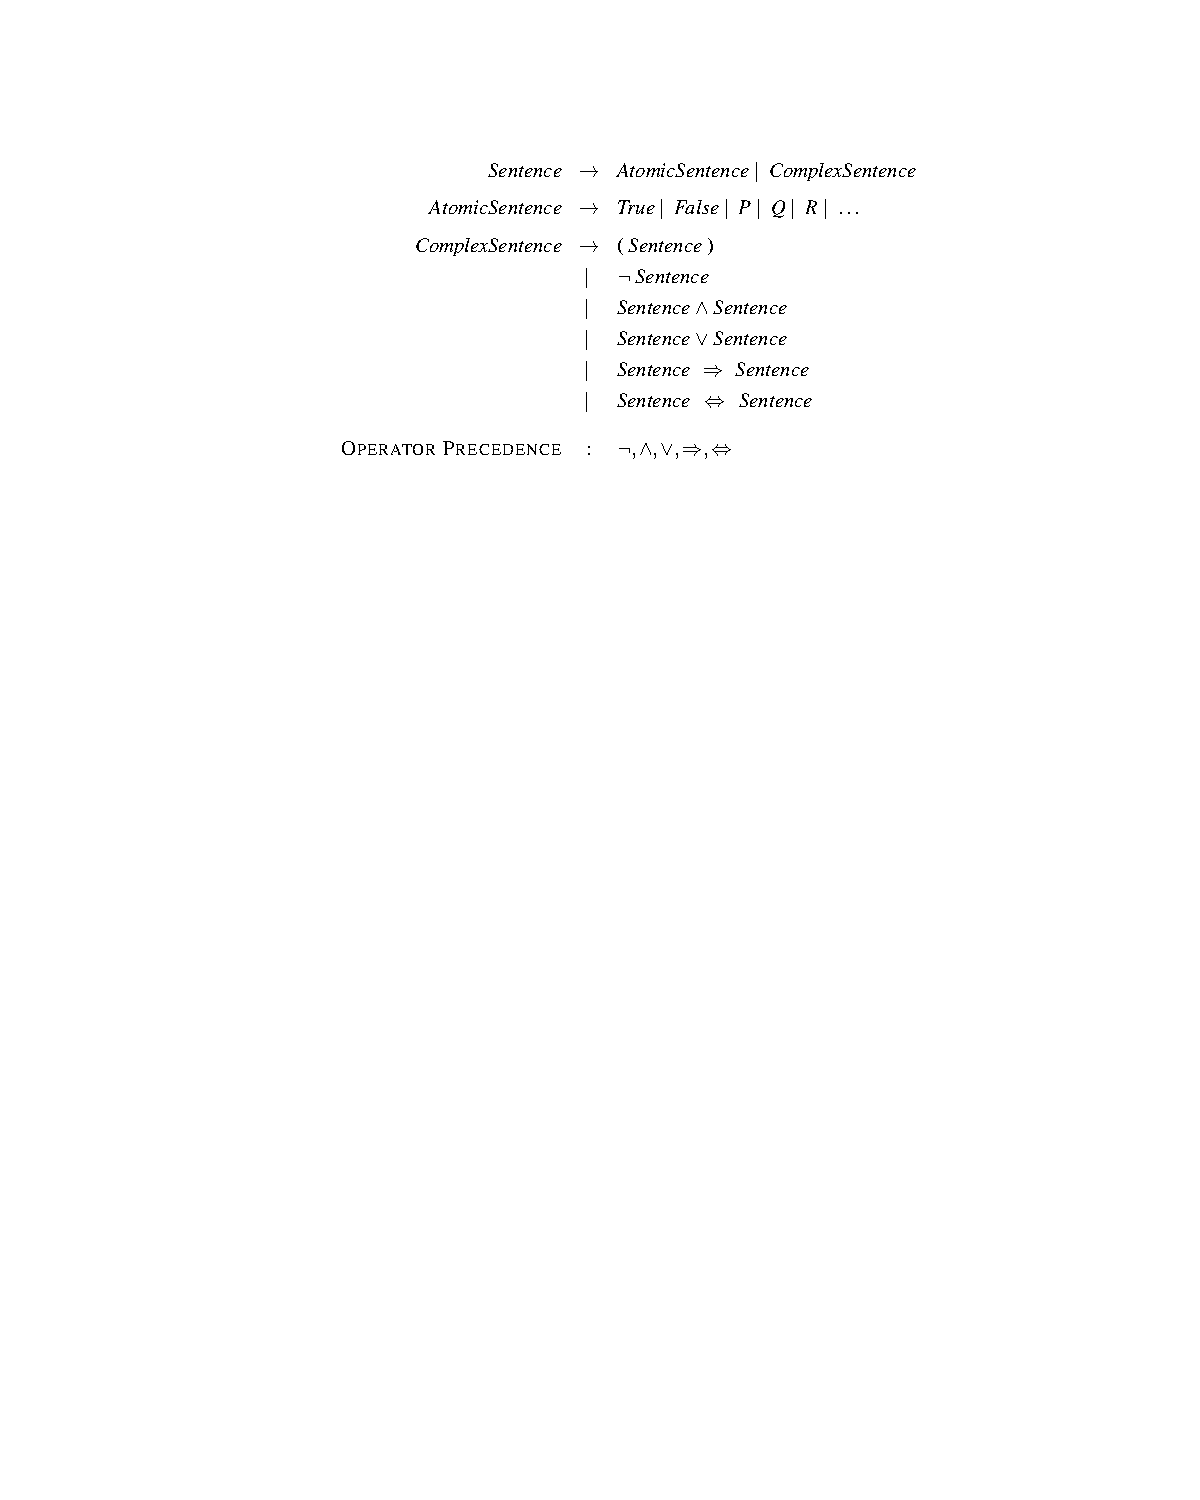
\includegraphics[alt={aima fig 07_07 grammar of popositional logic},height=2.8in]{aima-fig-07_07-grammar-of-popositional-logic.pdf}
\section{Propositional Logic}
\label{sec:orgfb70bda}


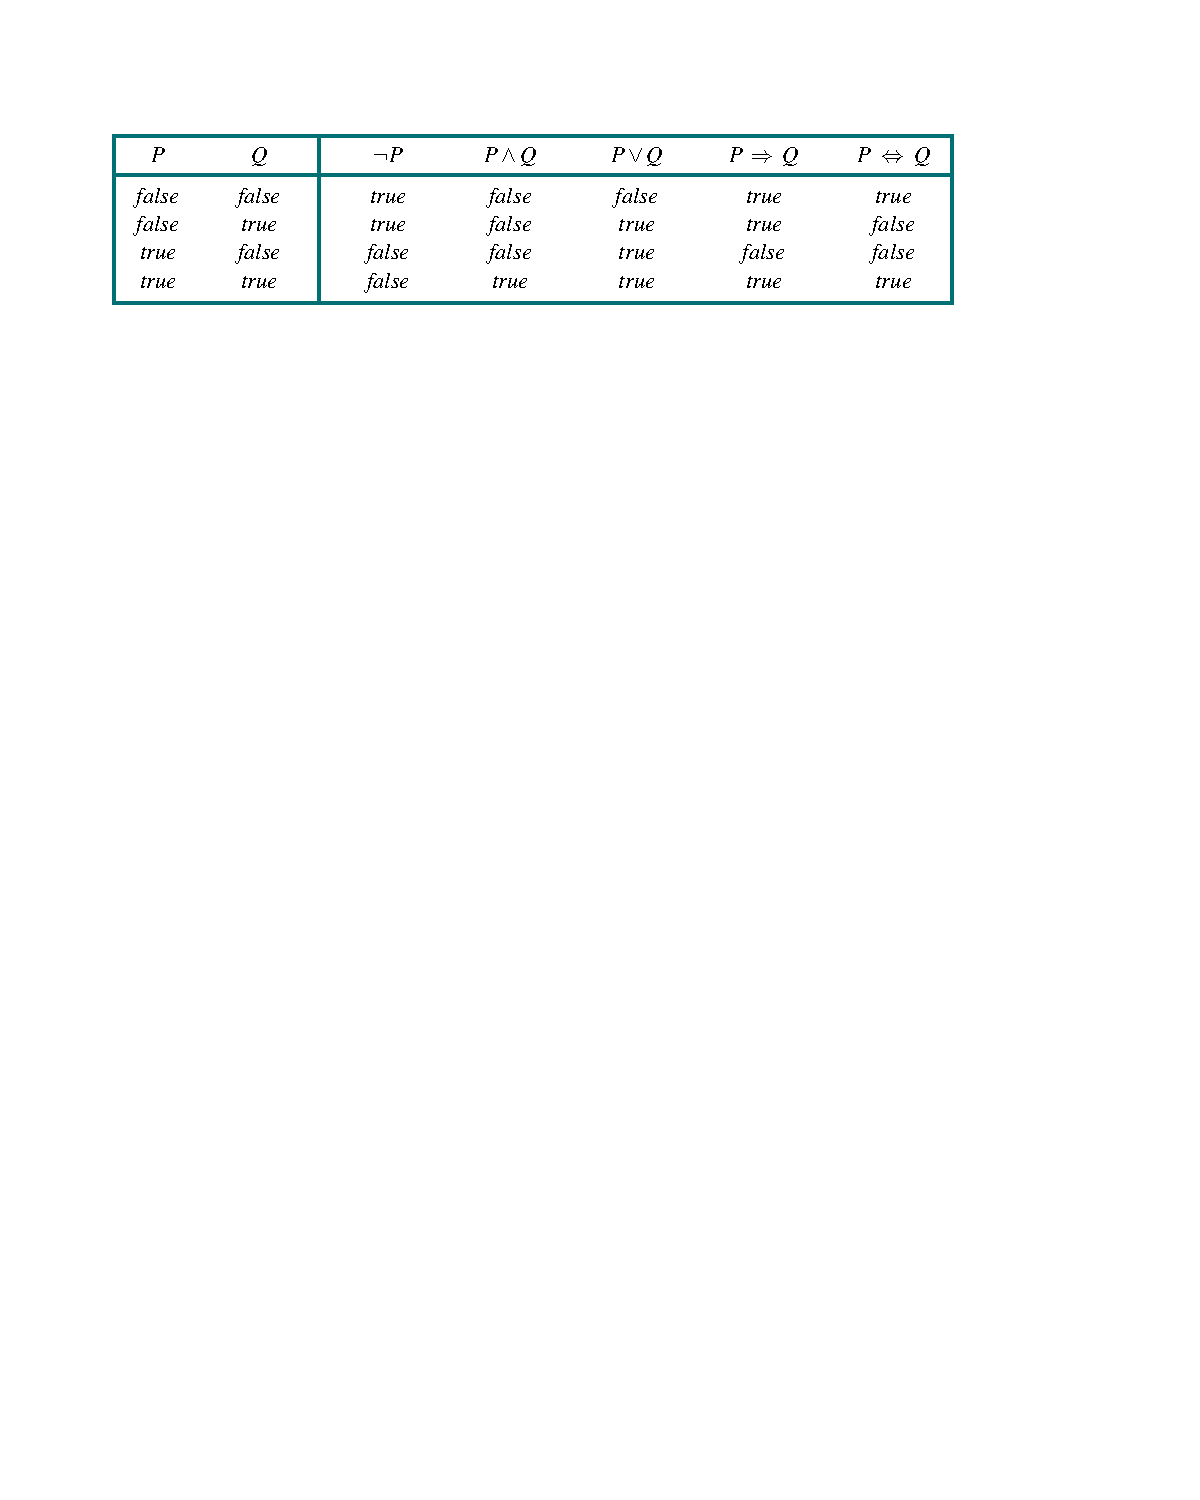
\includegraphics[alt={aima fig 07_08 truth tables logical connectives},height=2.8in]{aima-fig-07_08-truth-tables-logical-connectives.pdf}
\section{Propositional Theorem Proving}
\label{sec:org9a38800}


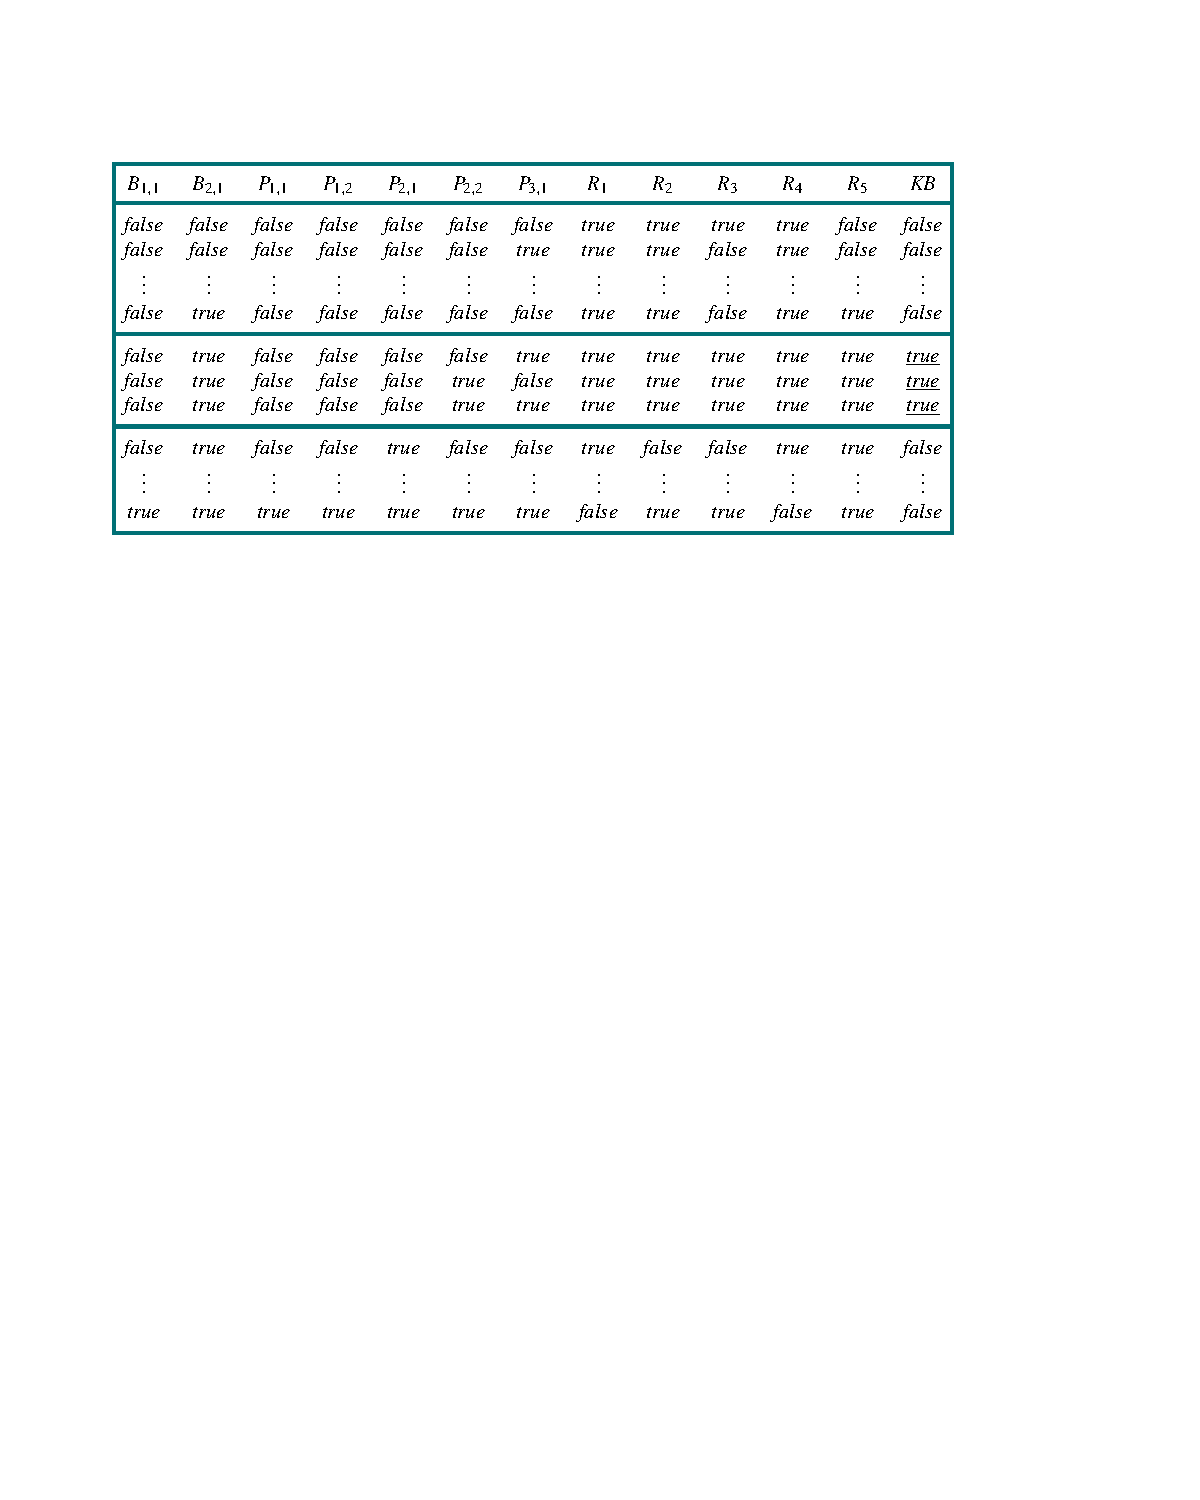
\includegraphics[alt={aima fig 07_09 truth table knowledge base},height=2.8in]{aima-fig-07_09-truth-table-knowledge-base.pdf}
\section{Propositional Theorem Proving}
\label{sec:org76ce22c}


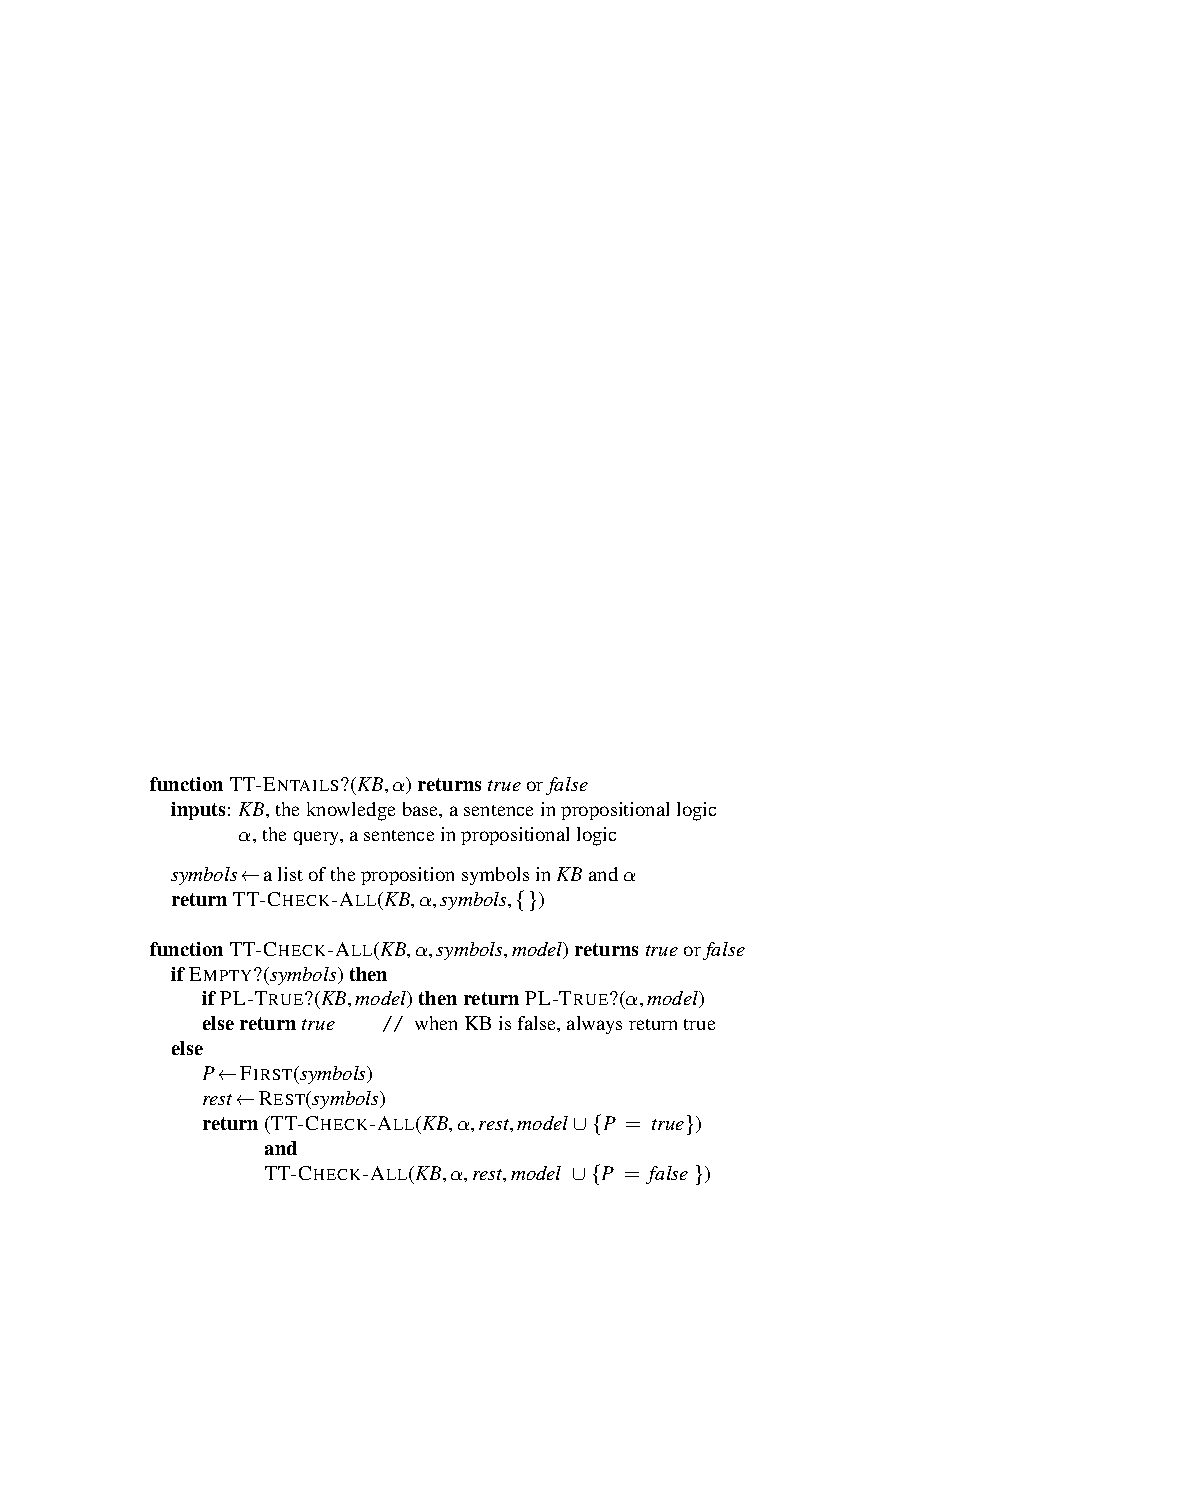
\includegraphics[alt={aima fig 07_10 tt entails algorithm},height=2.8in]{aima-fig-07_10-tt-entails-algorithm.pdf}
\section{Propositional Theorem Proving}
\label{sec:org33b0320}


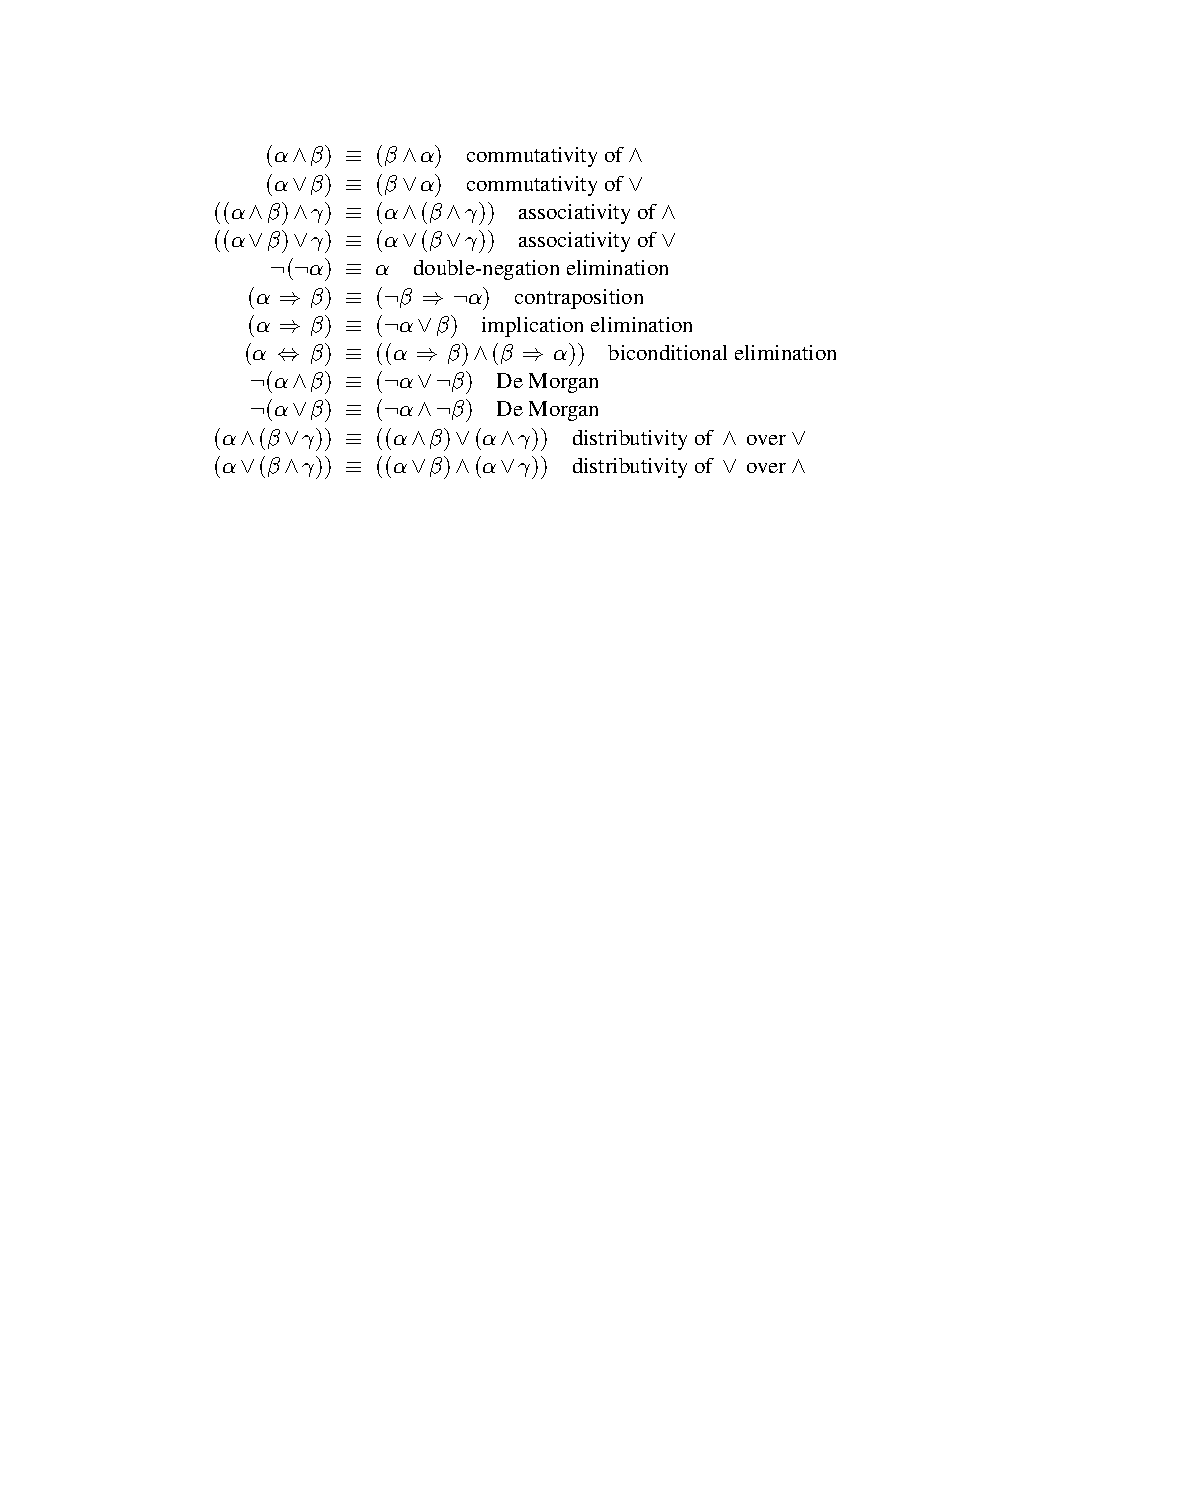
\includegraphics[alt={aima fig 07_11 logical equivalences},height=2.8in]{aima-fig-07_11-logical-equivalences.pdf}
\section{Propositional Theorem Proving}
\label{sec:orgd2ba3f7}


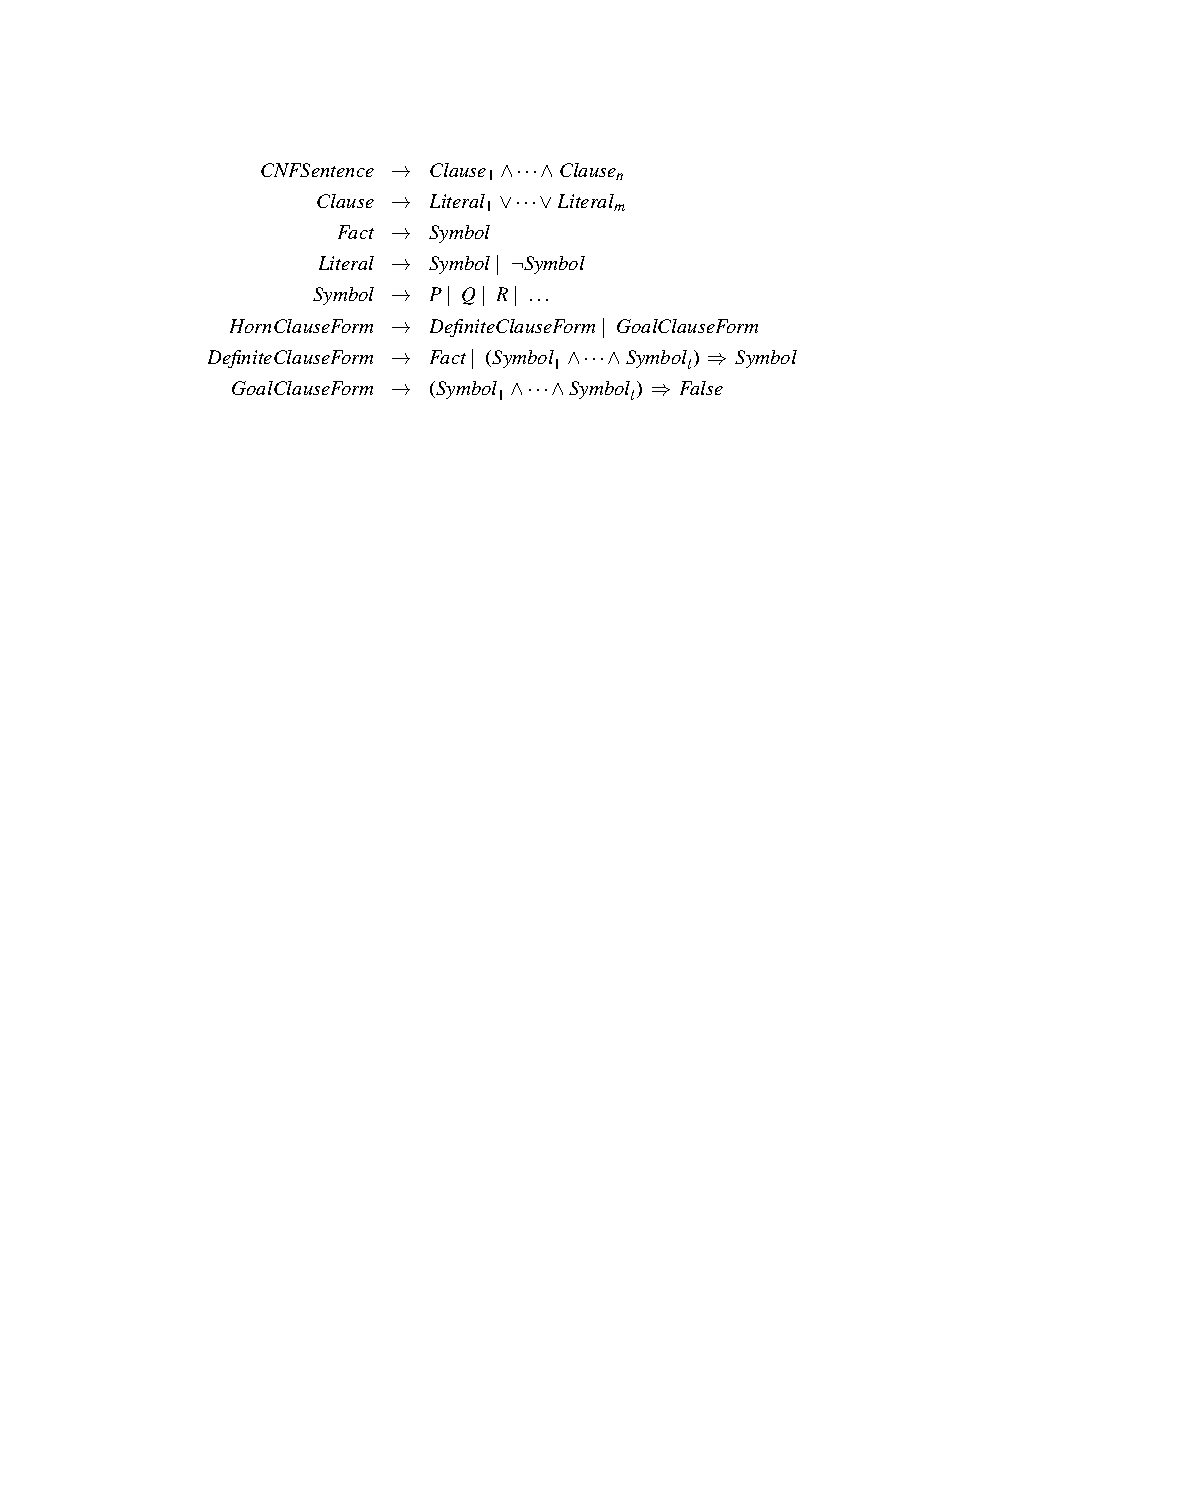
\includegraphics[alt={aima fig 07_12 grammar of cnf},height=2.8in]{aima-fig-07_12-grammar-of-cnf.pdf}
\section{Propositional Theorem Proving}
\label{sec:org97da112}


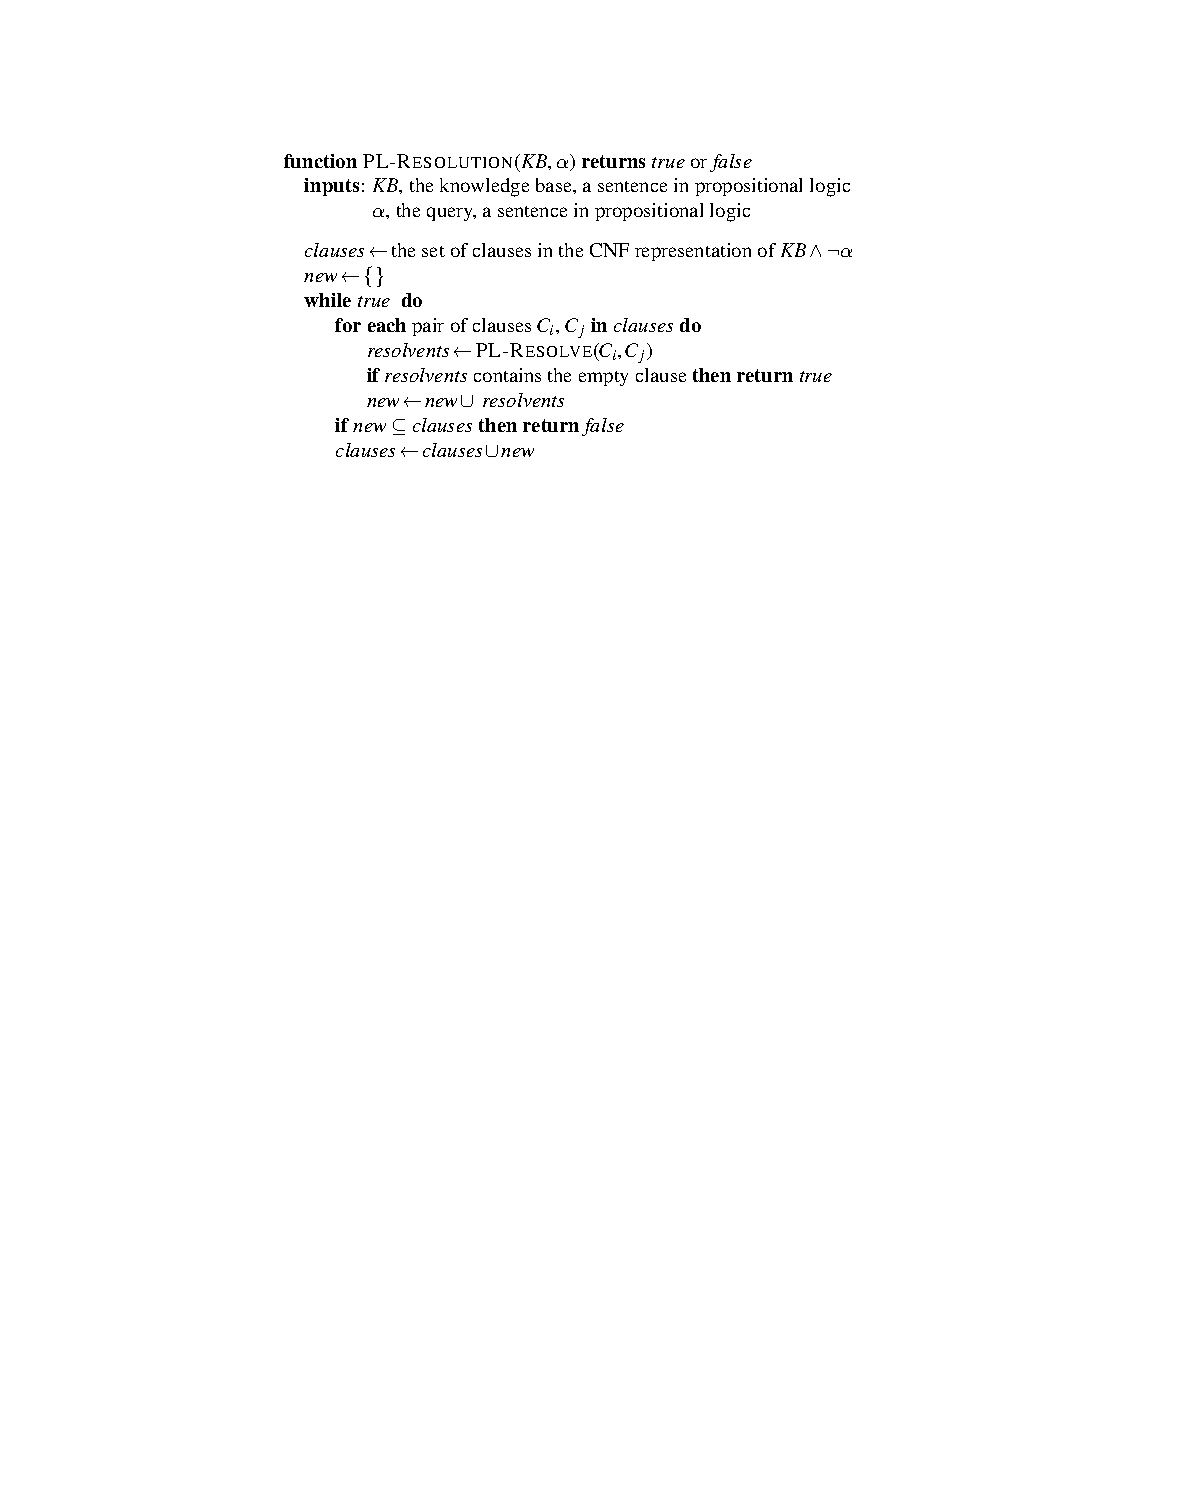
\includegraphics[alt={aima fig 07_13 pl resolution algorithm},height=2.8in]{aima-fig-07_13-pl-resolution-algorithm.pdf}
\section{Propositional Theorem Proving}
\label{sec:org833999f}


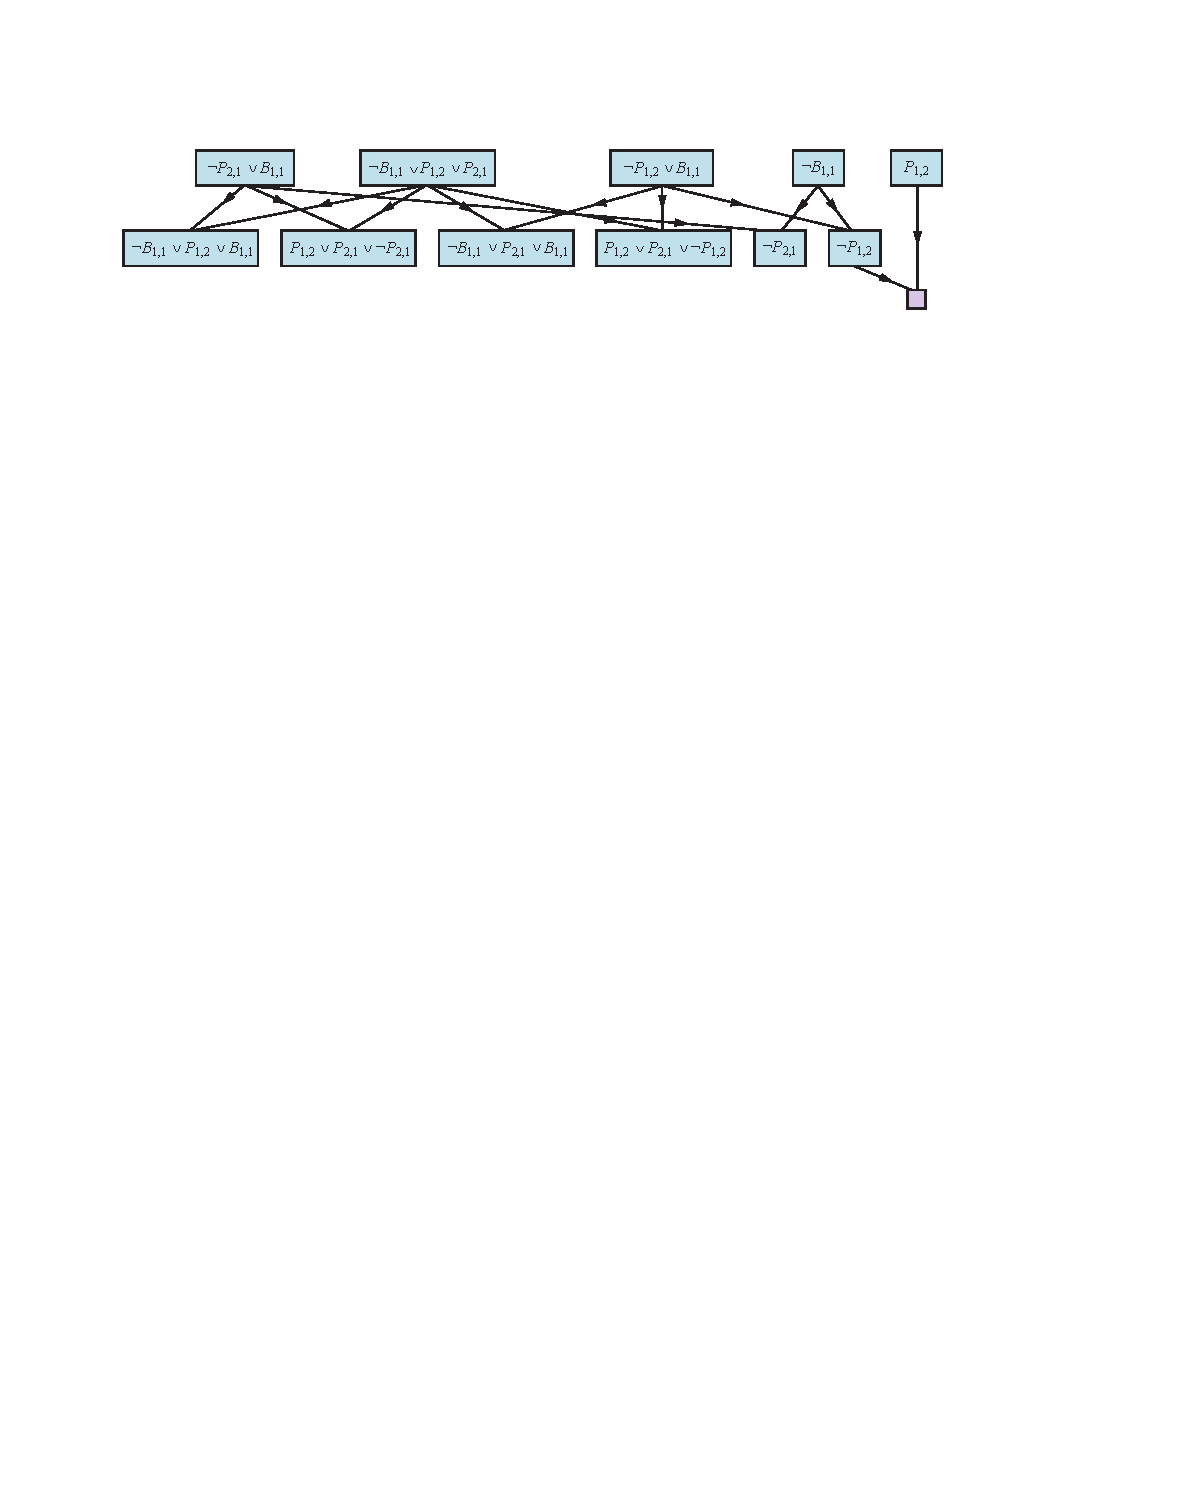
\includegraphics[alt={aima fig 07_14 pl resolution application},height=2.8in]{aima-fig-07_14-pl-resolution-application.pdf}
\section{Propositional Theorem Proving}
\label{sec:orge61efdd}


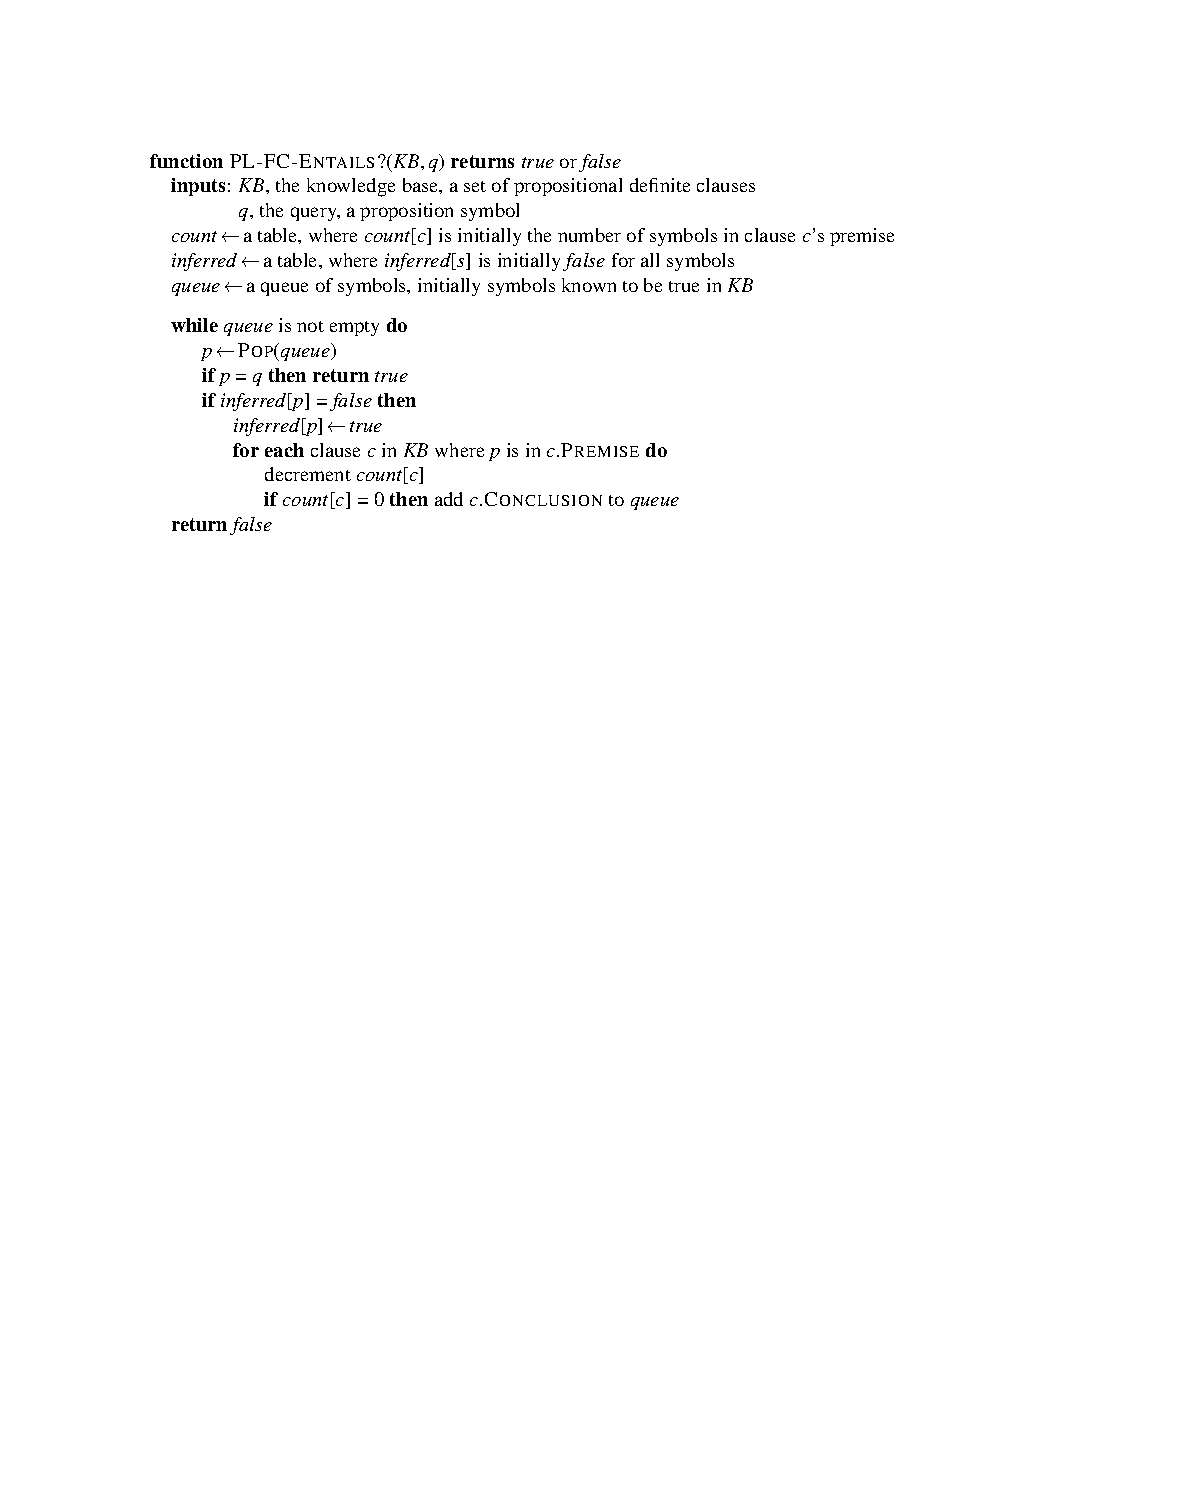
\includegraphics[alt={aima fig 07_15 pl fc entails algorithm},height=2.8in]{aima-fig-07_15-pl-fc-entails-algorithm.pdf}
\section{Propositional Theorem Proving}
\label{sec:org96701f4}


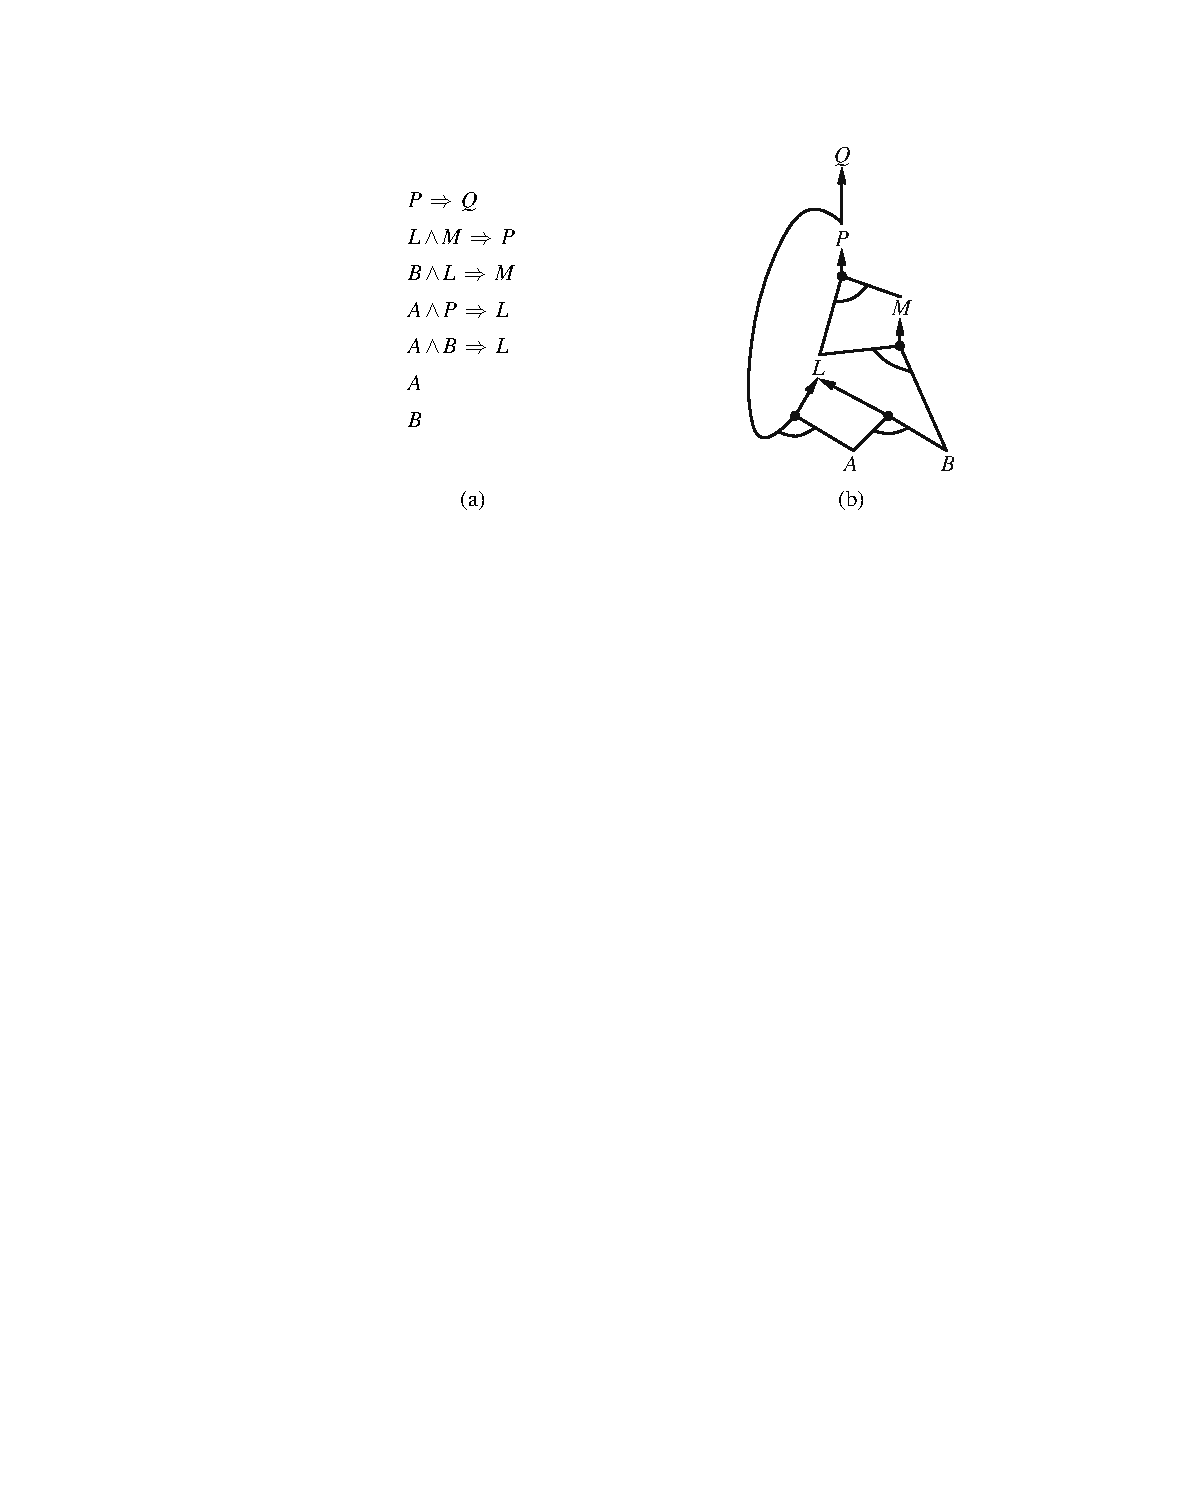
\includegraphics[alt={aima fig 07_16 horn clauses and or graph},height=2.8in]{aima-fig-07_16-horn-clauses-and-or-graph.pdf}
\section{Propositional Model Checking}
\label{sec:org2c9f4f0}


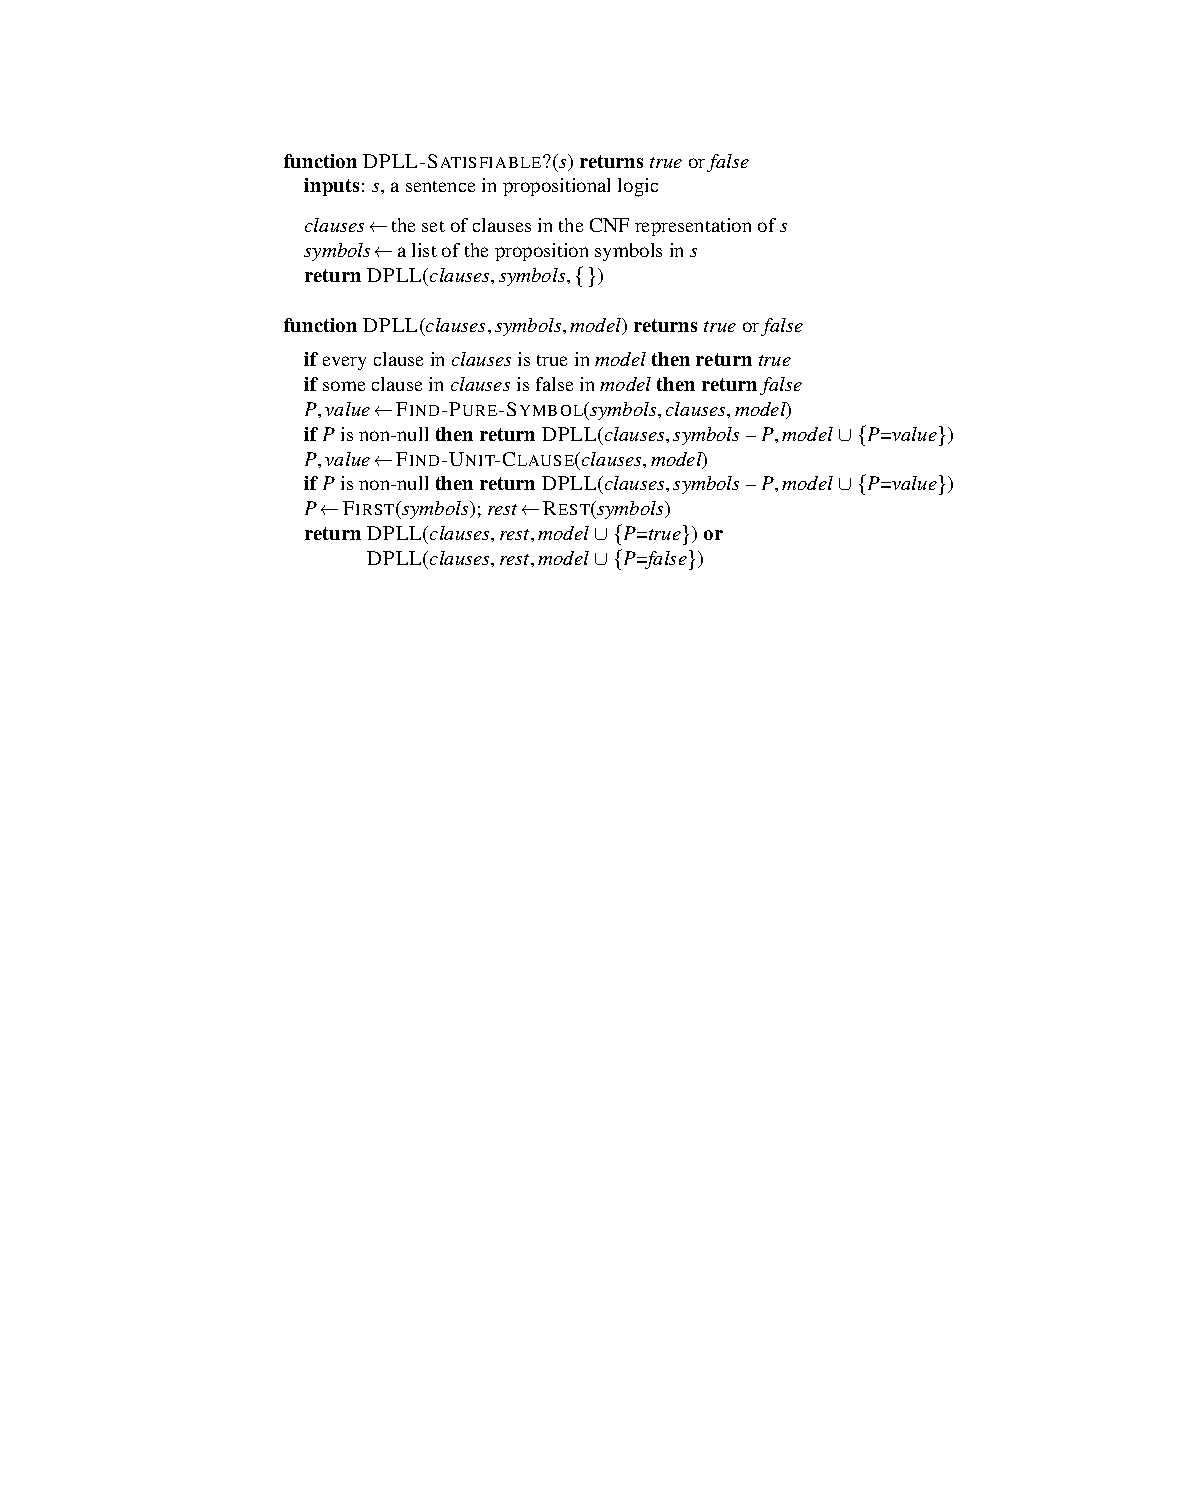
\includegraphics[alt={aima fig 07_17 dpll algorithm},height=2.8in]{aima-fig-07_17-dpll-algorithm.pdf}
\section{Propositional Model Checking}
\label{sec:org94a78a7}


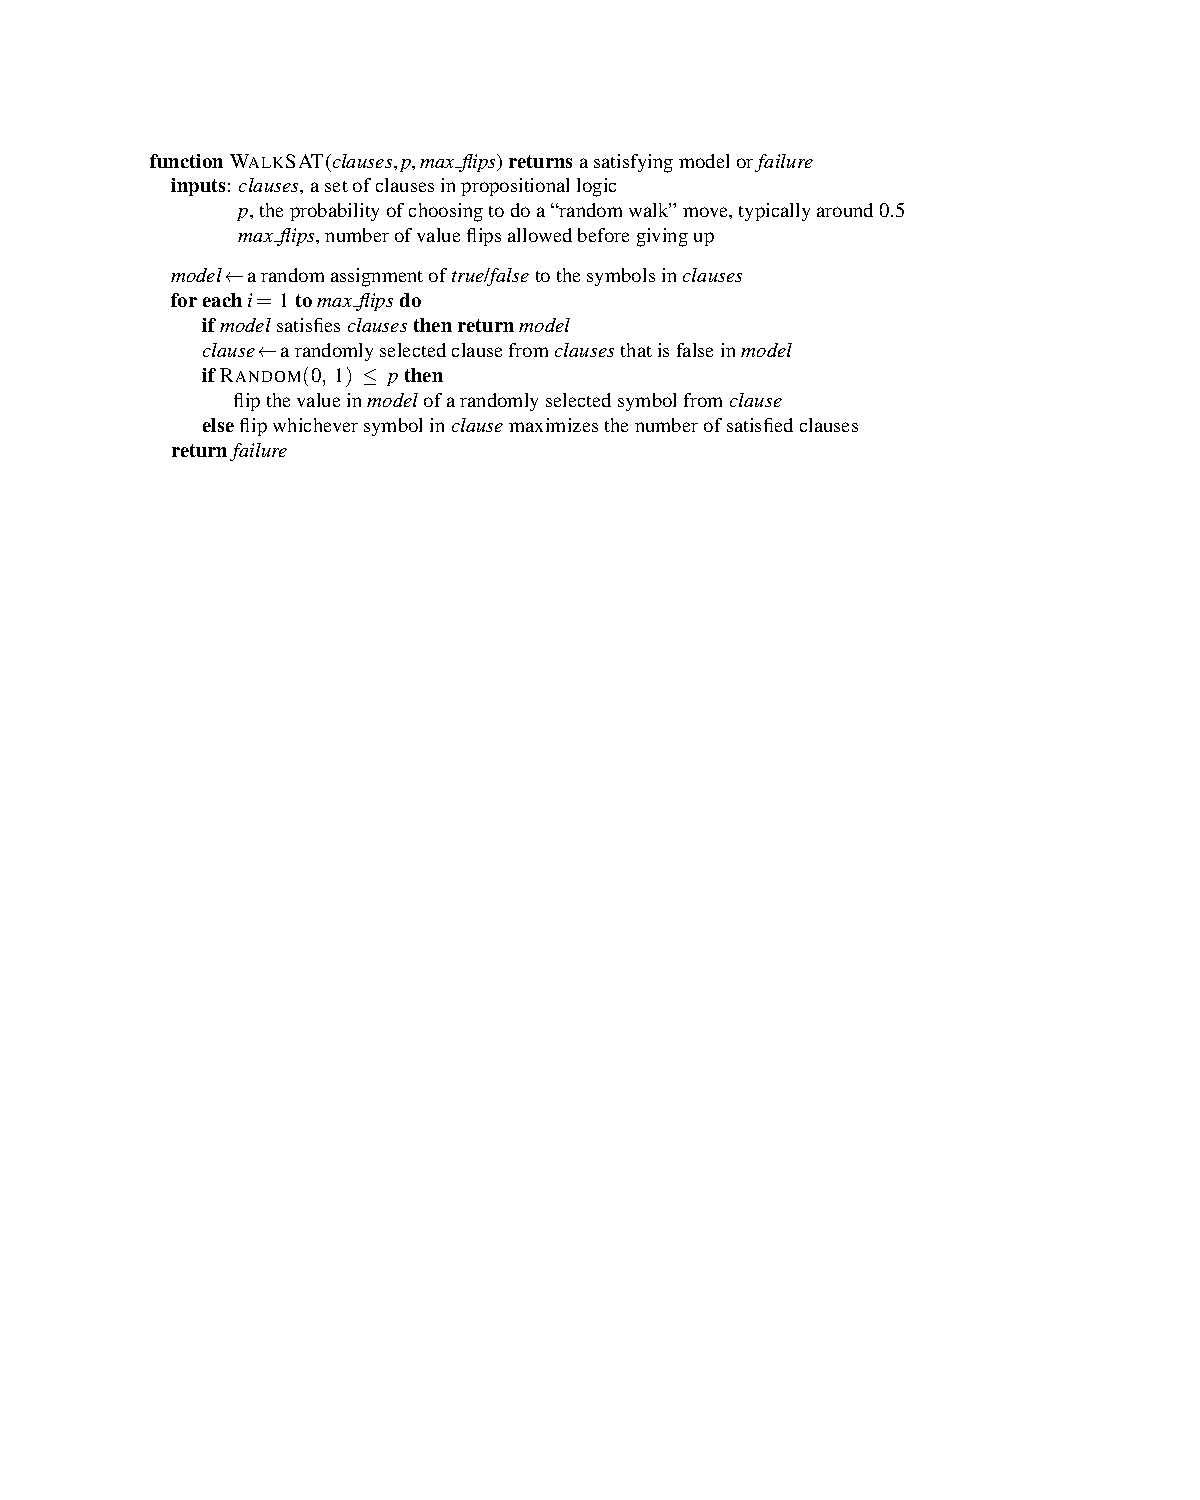
\includegraphics[alt={aima fig 07_18 walksat algorithm},height=2.8in]{aima-fig-07_18-walksat-algorithm.pdf}
\section{Propositional Model Checking}
\label{sec:orgb94a130}


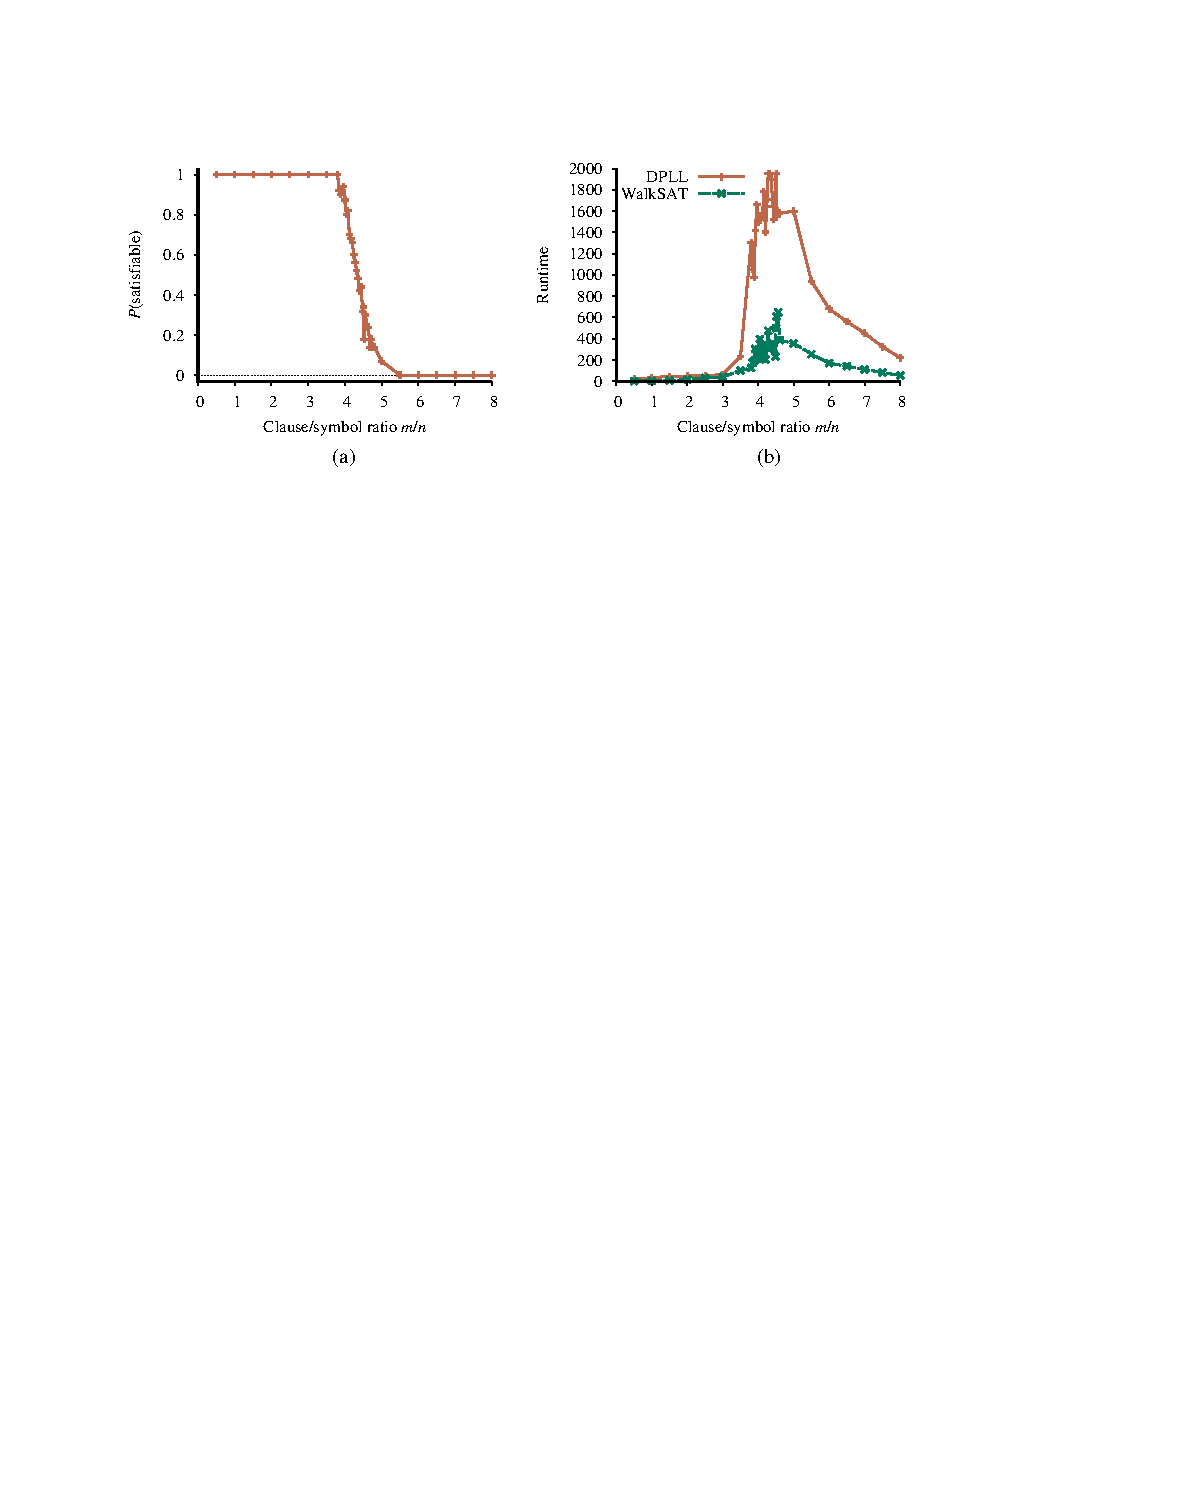
\includegraphics[alt={aima fig 07_19 dpll vs walksat},height=2.8in]{aima-fig-07_19-dpll-vs-walksat.pdf}
\section{Agents Based on Propositional Logic}
\label{sec:org0c42c70}


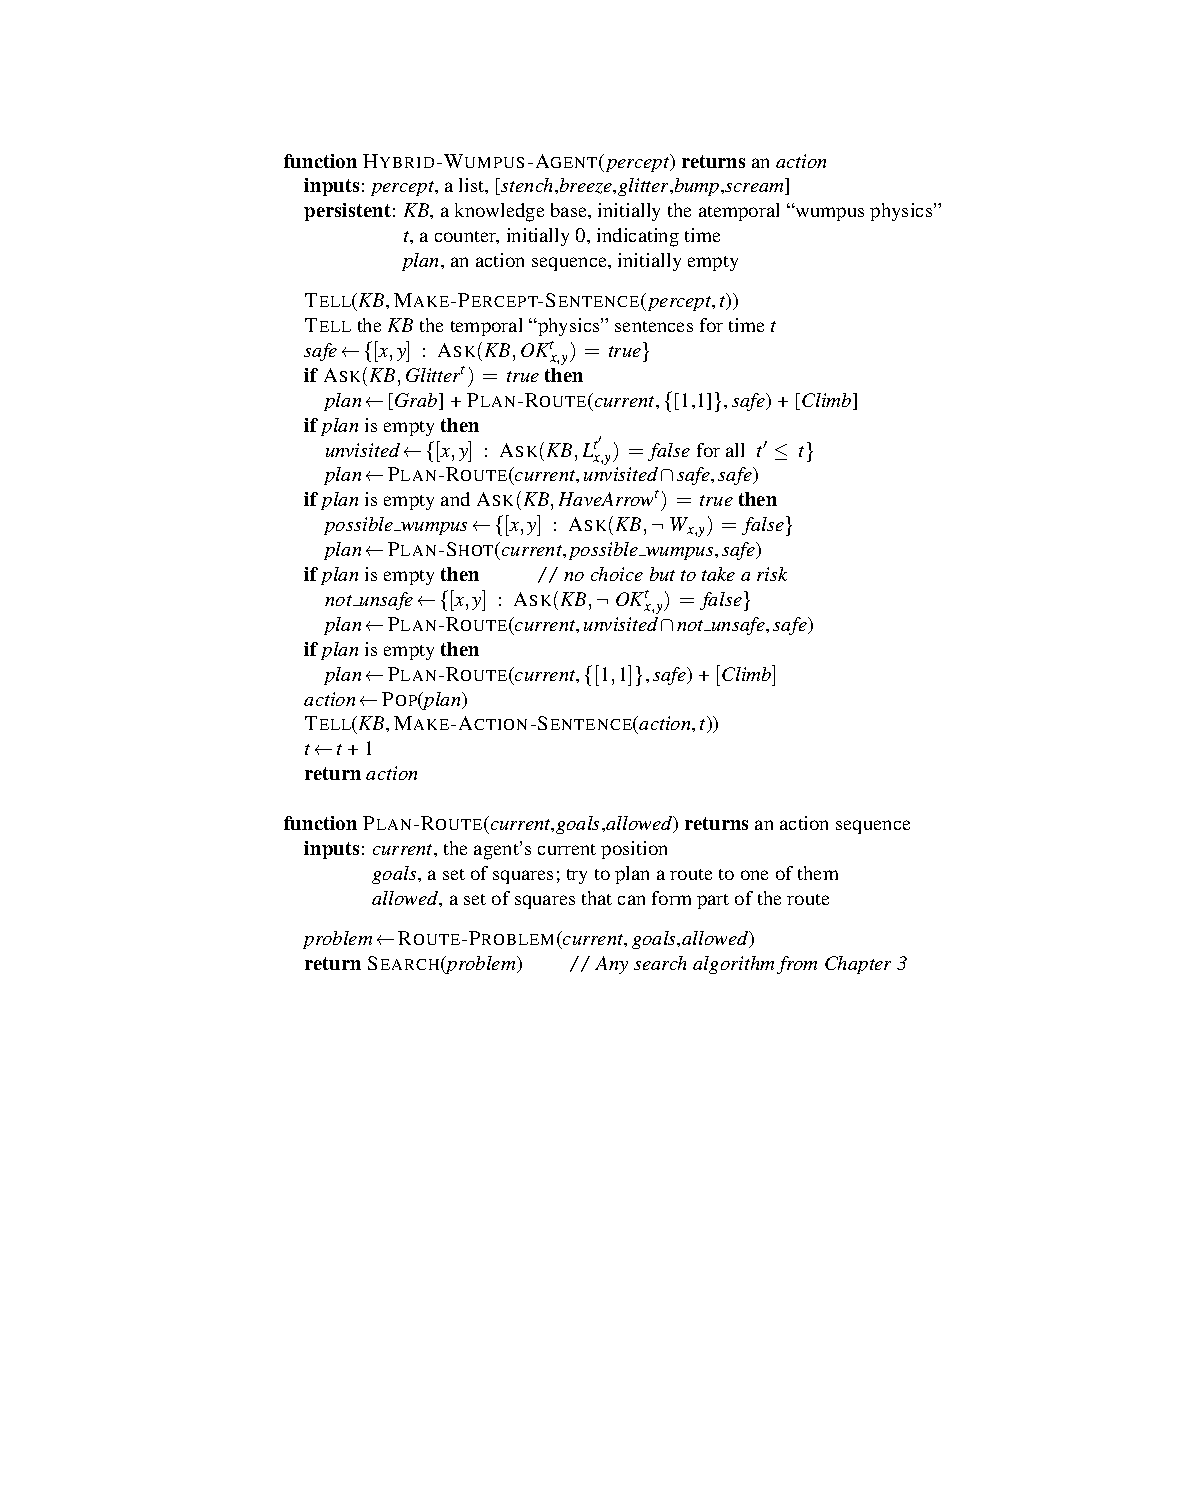
\includegraphics[alt={aima fig 07_20 hybrid wumpus agent algorithm},height=2.8in]{aima-fig-07_20-hybrid-wumpus-agent-algorithm.pdf}
\section{Agents Based on Propositional Logic}
\label{sec:org82e2405}


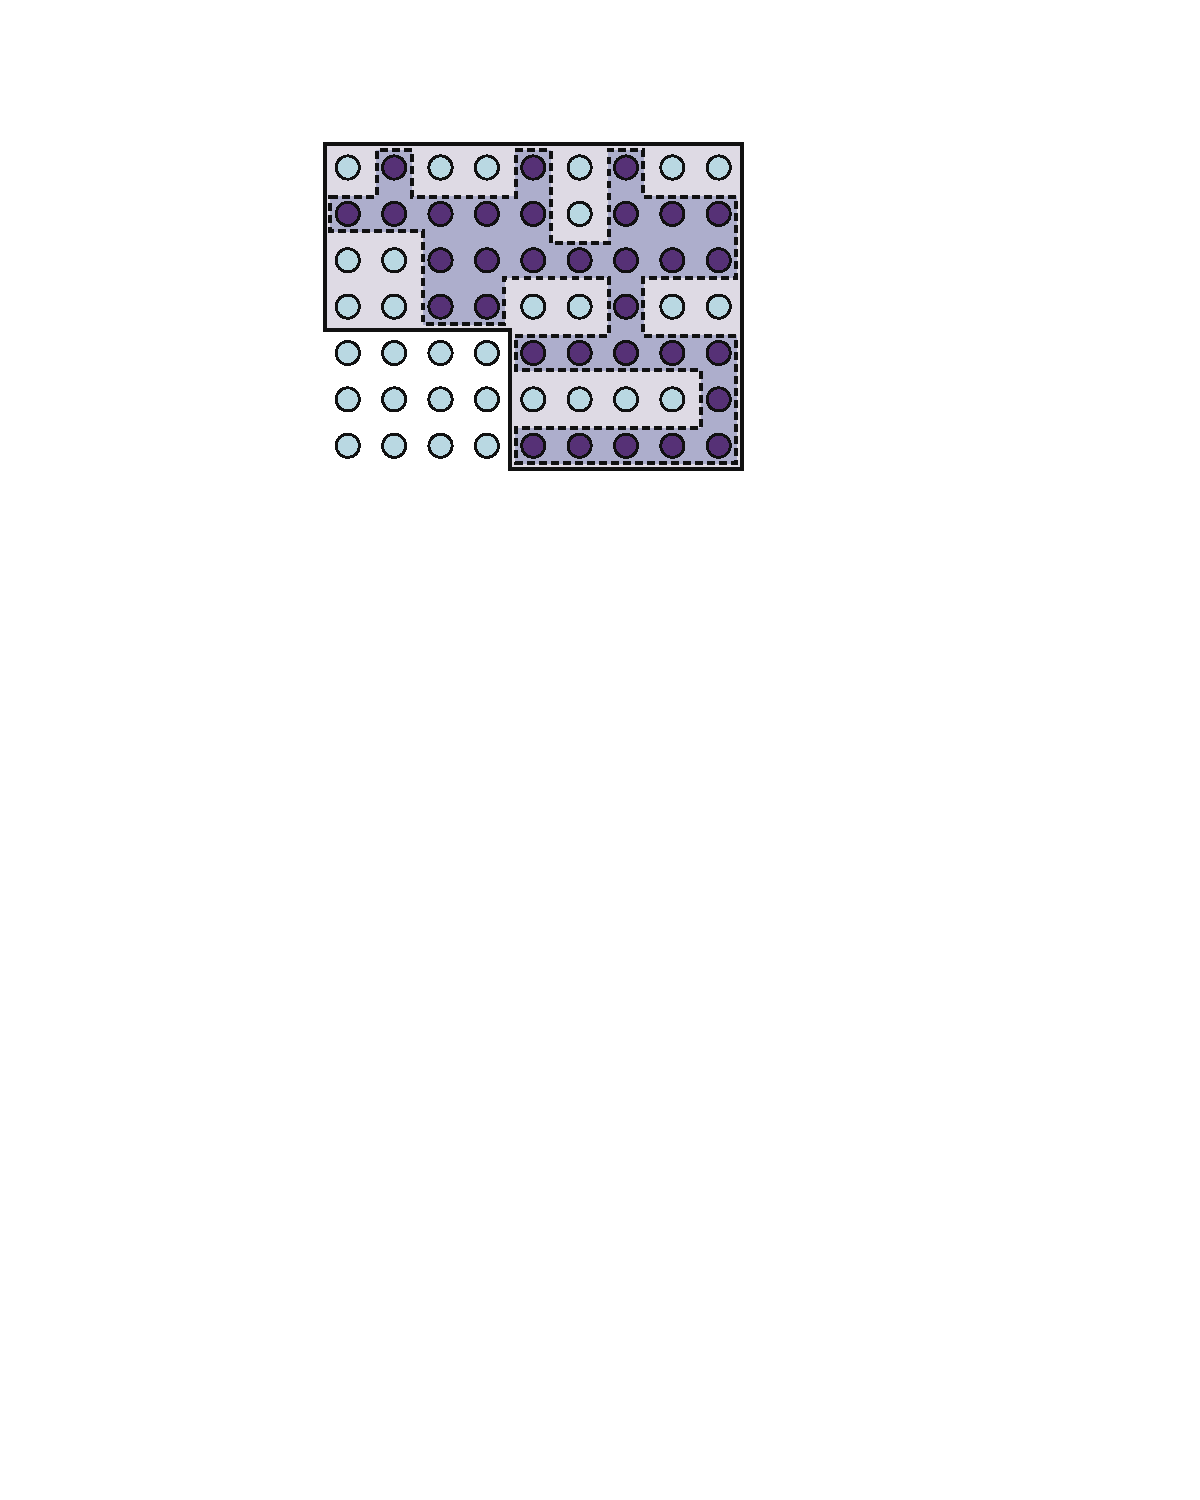
\includegraphics[alt={aima fig 07_21 1 cnf belief state},height=2.8in]{aima-fig-07_21-1-cnf-belief-state.pdf}
\section{Agents Based on Propositional Logic}
\label{sec:orged4aa2b}


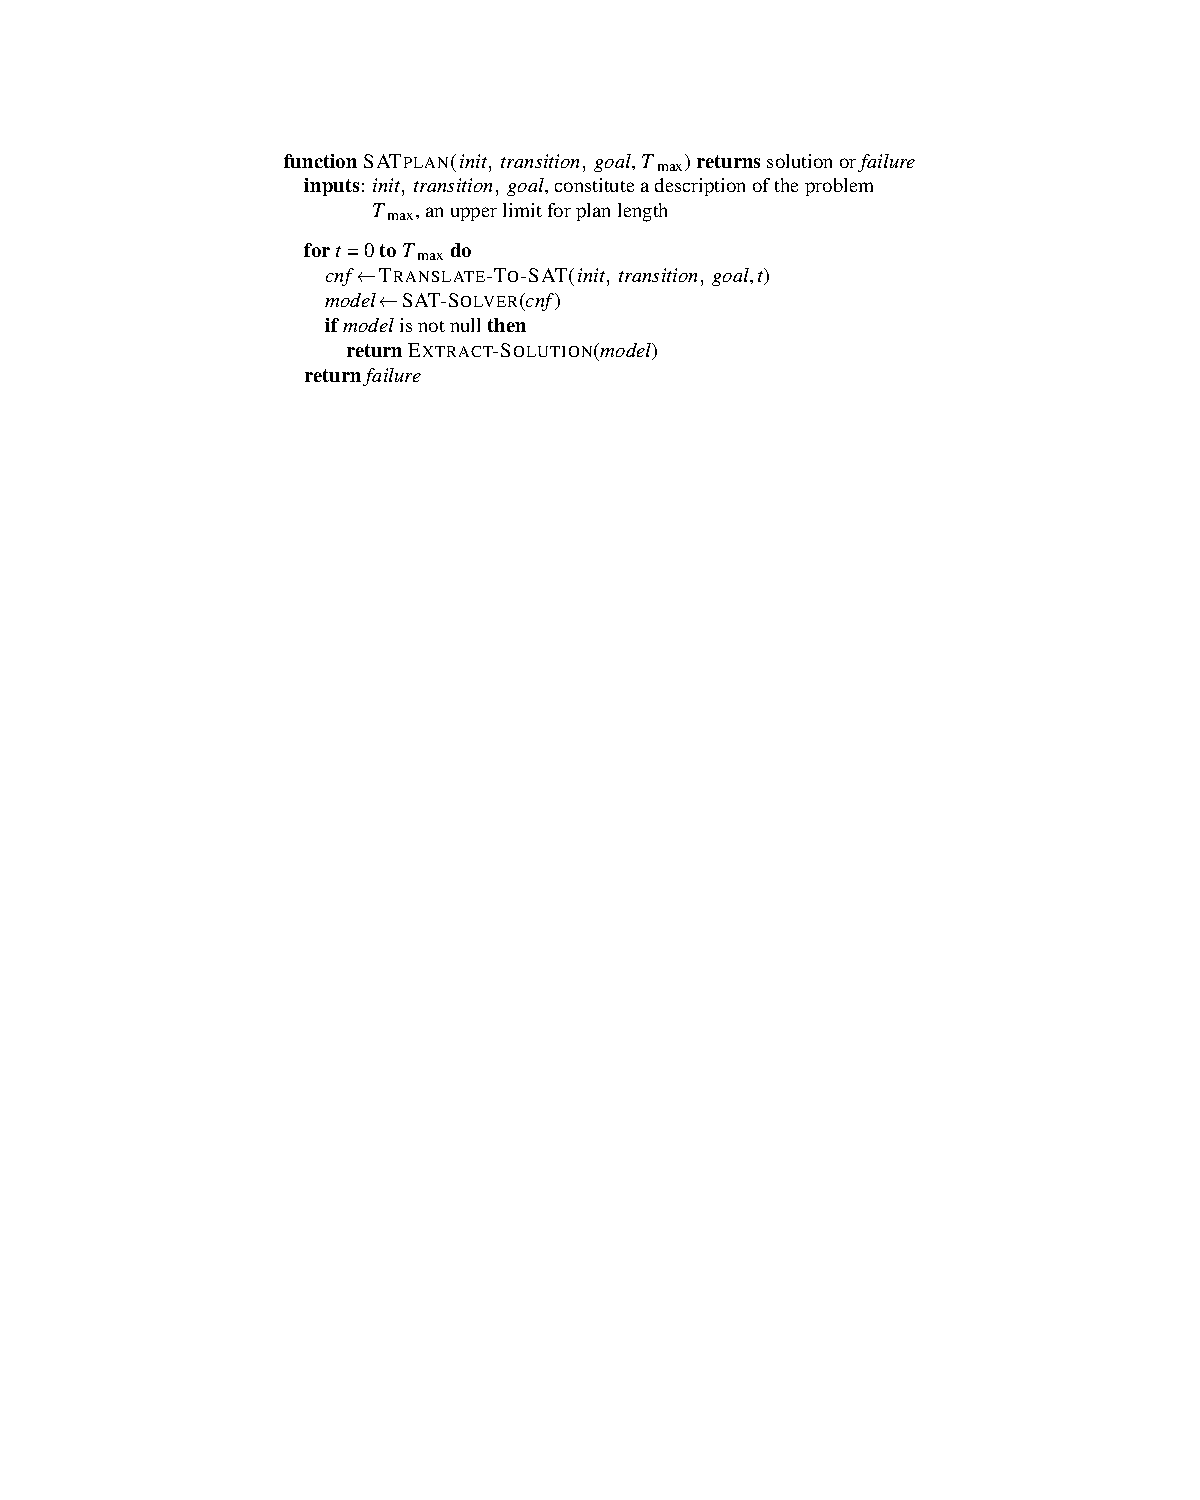
\includegraphics[alt={aima fig 07_22 satplan algorithm},height=2.8in]{aima-fig-07_22-satplan-algorithm.pdf}
\end{document}
